%  A simple AAU report template.
%  2015-05-08 v. 1.2.0
%  Copyright 2010-2015 by Jesper Kjær Nielsen <jkn@es.aau.dk>
%
%  This is free software: you can redistribute it and/or modify
%  it under the terms of the GNU General Public License as published by
%  the Free Software Foundation, either version 3 of the License, or
%  (at your option) any later version.
%
%  This is distributed in the hope that it will be useful,
%  but WITHOUT ANY WARRANTY; without even the implied warranty of
%  MERCHANTABILITY or FITNESS FOR A PARTICULAR PURPOSE.  See the
%  GNU General Public License for more details.
%
%  You can find the GNU General Public License at <http://www.gnu.org/licenses/>.
%
\usepackage{graphicx,hyperref,amsmath,bm,url}
\usepackage[numbers]{natbib}
\usepackage{microtype,todonotes}
\usepackage[danish]{babel}
\usepackage{a4}
\usepackage[compact,small]{titlesec}
\usepackage[utf8]{inputenc}
\clubpenalty = 10000
\widowpenalty = 10000
\usepackage[T1]{fontenc}
\graphicspath{ {../Billeder/} }
\usepackage{tikz}
\usetikzlibrary{calc}
\usetikzlibrary{shapes}

\makeatletter
\newdimen\@myBoxHeight%
\newdimen\@myBoxDepth%
\newdimen\@myBoxWidth%
\newdimen\@myBoxSize%
\newcommand{\SquareBox}[2][]{%
    \settoheight{\@myBoxHeight}{#2}% Record height of box
    \settodepth{\@myBoxDepth}{#2}% Record depth of box
    \settowidth{\@myBoxWidth}{#2}% Record width of box
    \pgfmathsetlength{\@myBoxSize}{max(\@myBoxWidth,(\@myBoxHeight+\@myBoxDepth))}%
    \tikz \node [shape=rectangle, shape aspect=1,draw=red,inner sep=2\pgflinewidth, minimum size=\@myBoxSize,#1] {#2};%
}%
\makeatother
\newcommand*{\captionsource}[2]{%
  \caption[{#1}]{%
    #1%
    \\\hspace{\linewidth}%
    \textbf{Kilde:} #2%
  }%
}% package inclusion and set up of the document
% see, e.g., http://en.wikibooks.org/wiki/LaTeX/Formatting#Hyphenation
% for more information on word hyphenation
\hyphenation{ex-am-ple hy-phen-a-tion short}
\hyphenation{long la-tex}
% 
%  A simple AAU report template.
%  2015-05-08 v. 1.2.0
%  Copyright 2010-2015 by Jesper Kjær Nielsen <jkn@es.aau.dk>
%
%  This is free software: you can redistribute it and/or modify
%  it under the terms of the GNU General Public License as published by
%  the Free Software Foundation, either version 3 of the License, or
%  (at your option) any later version.
%
%  This is distributed in the hope that it will be useful,
%  but WITHOUT ANY WARRANTY; without even the implied warranty of
%  MERCHANTABILITY or FITNESS FOR A PARTICULAR PURPOSE.  See the
%  GNU General Public License for more details.
%
%  You can find the GNU General Public License at <http://www.gnu.org/licenses/>.
%
%
%
% see, e.g., http://en.wikibooks.org/wiki/LaTeX/Customizing_LaTeX#New_commands
% for more information on how to create macros

%%%%%%%%%%%%%%%%%%%%%%%%%%%%%%%%%%%%%%%%%%%%%%%%
% Macros for the titlepage
%%%%%%%%%%%%%%%%%%%%%%%%%%%%%%%%%%%%%%%%%%%%%%%%
%Creates the aau titlepage
\newcommand{\aautitlepage}[3]{%
  {
    %set up various length
    \ifx\titlepageleftcolumnwidth\undefined
      \newlength{\titlepageleftcolumnwidth}
      \newlength{\titlepagerightcolumnwidth}
    \fi
    \setlength{\titlepageleftcolumnwidth}{0.5\textwidth-\tabcolsep}
    \setlength{\titlepagerightcolumnwidth}{\textwidth-2\tabcolsep-\titlepageleftcolumnwidth}
    %create title page
    \thispagestyle{empty}
    \noindent%
    \begin{tabular}{@{}ll@{}}
      \parbox{\titlepageleftcolumnwidth}{
        \iflanguage{danish}{%
          \includegraphics[width=\titlepageleftcolumnwidth]{aau_logo_da}
        }{%
          
\includegraphics[width=\titlepageleftcolumnwidth]{aau_logo_en}
        }
      } &
      \parbox{\titlepagerightcolumnwidth}{\raggedleft\sf\small
        #2
      }\bigskip\\
       #1 &
      \parbox[t]{\titlepagerightcolumnwidth}{%
      \textbf{Abstract:}\bigskip\par
        \fbox{\parbox{\titlepagerightcolumnwidth-2\fboxsep-2\fboxrule}{%
          #3
        }}
      }\\
    \end{tabular}
    \vfill
    \iflanguage{danish}{%
      \noindent{\footnotesize\emph{Rapportens indhold er frit tilgængeligt, men offentliggørelse (med kildeangivelse) må kun ske efter aftale med forfatterne.}}
    }{%
      \vspace{1mm}\noindent{\footnotesize\emph{The content of this report is freely available, but publication (with reference) may only be pursued due to agreement with the author.}}
    }
    \clearpage
  }
}

%Create english project info
\newcommand{\englishprojectinfo}[8]{%
  \parbox[t]{\titlepageleftcolumnwidth}{
    \textbf{Title:}\\ #1\bigskip\par
    \textbf{Theme:}\\ #2\bigskip\par
    \textbf{Project Period:}\\ #3\bigskip\par
    \textbf{Project Group:}\\ #4\bigskip\par
    \textbf{Participant(s):}\\ #5\bigskip\par
    \textbf{Supervisor(s):}\\ #6\bigskip\par
    \textbf{Copies:} #7\bigskip\par
    \textbf{Page Numbers:} \pageref{LastPage}\bigskip\par
    \textbf{Date of Completion:}\\ #8
  }
}

%Create danish project info
\newcommand{\danishprojectinfo}[8]{%
  \parbox[t]{\titlepageleftcolumnwidth}{
    \textbf{Titel:}\\ #1\bigskip\par
    \textbf{Tema:}\\ #2\bigskip\par
    \textbf{Projektperiode:}\\ #3\bigskip\par
    \textbf{Projektgruppe:}\\ #4\bigskip\par
    \textbf{Deltager(e):}\\ #5\bigskip\par
    \textbf{Vejleder(e):}\\ #6\bigskip\par
    \textbf{Oplagstal:} #7\bigskip\par
    \textbf{Sidetal:} \pageref{LastPage}\bigskip\par
    \textbf{Afleveringsdato:}\\ #8
  }
}

%%%%%%%%%%%%%%%%%%%%%%%%%%%%%%%%%%%%%%%%%%%%%%%%
% An example environment
%%%%%%%%%%%%%%%%%%%%%%%%%%%%%%%%%%%%%%%%%%%%%%%%
\theoremheaderfont{\normalfont\bfseries}
\theorembodyfont{\normalfont}
\theoremstyle{break}
\def\theoremframecommand{{\color{gray!50}\vrule width 5pt \hspace{5pt}}}
\newshadedtheorem{exa}{Example}[chapter]
\newenvironment{example}[1]{%
		\begin{exa}[#1]
}{%
		\end{exa}
}
% my new macros

\begin{document}
%frontmatter
\pagestyle{empty} %disable headers and footers
\pagenumbering{roman} %use roman page numbering in the frontmatter
%  A simple AAU report template.
%  2015-05-08 v. 1.2.0
%  Copyright 2010-2015 by Jesper Kjær Nielsen <jkn@es.aau.dk>
%
%  This is free software: you can redistribute it and/or modify
%  it under the terms of the GNU General Public License as published by
%  the Free Software Foundation, either version 3 of the License, or
%  (at your option) any later version.
%
%  This is distributed in the hope that it will be useful,
%  but WITHOUT ANY WARRANTY; without even the implied warranty of
%  MERCHANTABILITY or FITNESS FOR A PARTICULAR PURPOSE.  See the
%  GNU General Public License for more details.
%
%  You can find the GNU General Public License at <http://www.gnu.org/licenses/>.
%
\pdfbookmark[0]{Front page}{label:frontpage}%
\begin{titlepage}
  \addtolength{\hoffset}{0.5\evensidemargin-0.5\oddsidemargin} %set equal margins on the frontpage - remove this line if you want default margins
  \noindent%
  \begin{tabular}{@{}p{\textwidth}@{}}
    \toprule[2pt]
    \midrule
    \vspace{0.2cm}
    \begin{center}
    \Huge{\textbf{
      Report Title% insert your title here
    }}
    \end{center}
    \begin{center}
      \Large{
        - Subtitle -% insert your subtitle here
      }
    \end{center}
    \vspace{0.2cm}\\
    \midrule
    \toprule[2pt]
  \end{tabular}
  \vspace{4 cm}
  \begin{center}
    {\large
      Project Report%Insert document type (e.g., Project Report)
    }\\
    \vspace{0.2cm}
    {\Large
      Group Name/Number%Insert your group name or real names here
    }
  \end{center}
  \vfill
  \begin{center}
  Aalborg University\\
  Electronics and IT
  \end{center}
\end{titlepage}
\clearpage

\thispagestyle{empty}
{\small
\strut\vfill % push the content to the bottom of the page
\noindent Copyright \copyright{} Aalborg University 2015\par
\vspace{0.2cm}
\noindent This report has been typeset using \LaTeX.
}
\clearpage


\pdfbookmark[0]{English title page}{label:titlepage_en}
\aautitlepage{%
  \englishprojectinfo{
    Hiding in Plain Sight - Using a Graph-theoretical Approach to Steganography for hiding data in JPEG images %title
  }{%
    Programming and Problem Solving %theme
  }{%
    Spring Semester 2016 %project period
  }{%
    DAT2-A423 % project group
  }{%
    %list of group members
    Henrik Herbst Sørensen \\
    Jacob Askløf Svenningsen\\
    Jakob Meldgaard Kjær\\
    Leo Johannesen Mohr\\
    Mathias Steen Jakobsen\\ 
    Søren Madsen\\
    Theresa Krogh-Walker
  }{%
    %list of supervisors
    Kurt Nørmark
  }{%
    2 % number of printed copies
  }{%
    \today % date of completion
  }%
}{%department and address
  \textbf{Department of Computer Science}\\
  Aalborg University\\
  \href{http://www.cs.aau.dk/}{http://www.cs.aau.dk/}
}{% the abstract
  This report contains an analysis of the problem with Steganography and how it can be detected through Steganalysis. 
  It'll also give some insight in something more contextual, such as if it can be used in Social Media by rebels who lives under a tyrannical regime and whom wishes to communicate with one another, without being detected and risk being executed.
   During the report, some steganographic experiments has been conducted, and the image format known as JPEG, which is by far, the most used format when it comes to sharing images on the internet, has been thoroughly analysed, and the programme which has been developed during the writing of this report, has been designed to work on that very format. 
   The programme is able to embed a message secretly within the image to make it as difficult to detect by the human eye as possible, using Graph Theory from the branch of Mathematics known as Discrete Mathematics. 
}

\cleardoublepage
\cleardoublepage
\pdfbookmark[0]{Contents}{label:contents}
\pagestyle{fancy} %enable headers and footers again
\tableofcontents
%\listoftodos
% -*- root: ../../DAT2-A423_Project_Report.tex -*-
\chapter*{Preface\markboth{Preface}{Preface}}\label{ch:preface}
\addcontentsline{toc}{chapter}{Preface}

\vspace{\baselineskip}\hfill Aalborg University, \today
\vfill\noindent

\begin{minipage}[b]{0.45\textwidth}
 \centering
 \rule{\textwidth}{0.5pt}\\
  Henrik Herbst Sørensen\\
 {\footnotesize hsaren14@student.aau.dk}
\end{minipage}
\hfill
\begin{minipage}[b]{0.45\textwidth}
 \centering
 \rule{\textwidth}{0.5pt}\\
 Jacob Askløf Svenningsen\\
 {\footnotesize jsvenn15@student.aau.dk}
\end{minipage}
\vspace{3\baselineskip}

\begin{minipage}[b]{0.45\textwidth}
 \centering
 \rule{\textwidth}{0.5pt}\\
  Jakob Meldgaard Kjær\\
 {\footnotesize jkjar14@student.aau.dk}
\end{minipage}
\hfill
\begin{minipage}[b]{0.45\textwidth}
 \centering
 \rule{\textwidth}{0.5pt}\\
  Leo Johannesen Mohr\\
 {\footnotesize lmohr15@student.aau.dk}
\end{minipage}
\vspace{3\baselineskip}

\begin{minipage}[b]{0.45\textwidth}
 \centering
 \rule{\textwidth}{0.5pt}\\
  Mathias Steen Jakobsen\\
 {\footnotesize msja15@student.aau.dk}
\end{minipage}
\hfill
\begin{minipage}[b]{0.45\textwidth}
 \centering
 \rule{\textwidth}{0.5pt}\\
  Søren Madsen\\
 {\footnotesize smads15@student.aau.dk}
\end{minipage}
\vspace{3\baselineskip}

\begin{center}
\begin{minipage}[b]{0.45\textwidth}
 \centering
 \rule{\textwidth}{0.5pt}
  Theresa Krogh-Walker\\
 {\footnotesize tkrogh15@student.aau.dk}
\end{minipage}
\end{center}

\cleardoublepage
%mainmatter
\pagenumbering{arabic} %use arabic page numbering in the mainmatter

% Main report
\chapter{Conclusion}\label{ch:conclusion}

	\section{Introduction to Steganography}
Through the ages, people have been dependent on efficient forms of communication. In some cases, these messages would include information that should ideally be confidential and not read by anyone else other than the intended recipient. To do this, would require a way of concealing the details of the message in a way that an outsider would not be able to decipher what the actual message is.

Whereas cryptography is about concealing a message's content in a way that reveals that a message is concealed(which would undoubtedly raise some form of suspicion), steganography is about concealing the message's existence. This means that instead of the private message's content being protected by an obvious security-measure, people have had to find ways of circumventing interception and hide their messages in plain view to avoid any suspicion. This is one advantage steganography has over cryptography. 

Steganography is the art of concealing a message in a cover object, without having other people being aware that the concealed message is being sent.\cite{Anderson1998} The cover object could be in the form of video, audio or plain text. An example of this could be, hiding information in something innocuous that is not likely to get any unwanted, extra attention. The concealment should be subtle, so that unless a person was aware there was something to be found, is very unlikely to notice that a message is being passed in front of them without their notice.

As not everyone wishes to have every detail of their life, scrutinised and under the watch of everyone, people have had to implement forms of steganography to get their meaning across to their intended recipient. This goes back centuries, for example, people in ancient China would write messages on fine silk, which would then be pressed together until it was a much smaller piece of material and covered in wax. The cover of this message, was a person who would have to swallow the message to bring the information safely, without interception to the intended receiver. \cite{Singh2001} Another example being medieval Europe, where they had a system using templates, which would then be placed over a text, highlighting what the actual message is.\cite{Anderson1998}

Since then, forms of steganography have become much more advanced, and naturally, digitalised. Steganography can be implemented by anyone, no matter their intention, but would most typically be people who feel like they have something to hide. With the rise of social media, sending messages via the internet, and specifically these social media networks, has become the norm. Therefore it is only natural that a modern form of steganography should be able to work on these platforms. 

	% -*- root: ../../DAT2-A423_Project_Report.tex -*-
\section{Discussion}
We started out by using the relatively simple LSB-method for hiding data in an image.
Specifically, we saved an image inside of another PNG-image.
While the differences in the image with and without the message-image were hardly noticeable to the human eye, we did find that comparing colour histograms of the two images revealed that there had in fact been made changes to it.
In an effort to diminish this problem, the graph-theoretical approach we implemented attempted to move pixels around in the image, rather than change their values.
This meant that colour histograms of the image before and after the message had been encoded should look very similar, almost identical.
Any changes would come from the unmatched pairs: the quantized DCT values used in the encoding that we did not find any interchangeable values for.
When this happened we were forced to change the individual values, which led to a change in the colour composition of the image.
Using this method, we expected the changes to be small enough so that it would not immediately draw attention to the image, if it was being subjected to a colour histogram.

\subsection{Changes to the image}
To find out roughly how many of these forces there were in a given image, we used our programme to save different messages in different images.
The used five different message lengths were: 70, 140, 280, 560 and 1120 bytes.
Each message consisted of the ASCII characters A-Z repeated to fill out the message.
Each of these messages were encoded in four images with varying motives, but the same resolution (1920x1080).
The images can be seen in figure \ref{fig:four_test_images}.

We used a cartoon-like drawing of a cat to see how our software would work on an image that was not ideal for the JPEG format.
The landscape image contained many different colours and very complex patterns, which made it ideal for JPEG compression.
The same could be said for the tiger, but it contained larger areas of similar colours than the landscape did.
The image of the snowy forest road contained very few colour nuances, but was almost entirely made up of the luminance channel.
This led to a total of 20 tests as seen in table \ref{fig:forces_swaps}.

\begin{figure}[H]
    \centering
    \begin{subfigure}[b]{0.33\textwidth}
        
\includegraphics[width=\textwidth]{figures/cat}
            \caption{Cat image}
    \end{subfigure}
    \begin{subfigure}[b]{0.33\textwidth}
            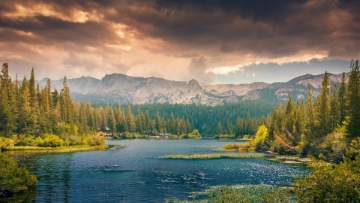
\includegraphics[width=\textwidth]{figures/landscape}
            \caption{Landscape image}
    \end{subfigure}
    \begin{subfigure}[b]{0.33\textwidth}
            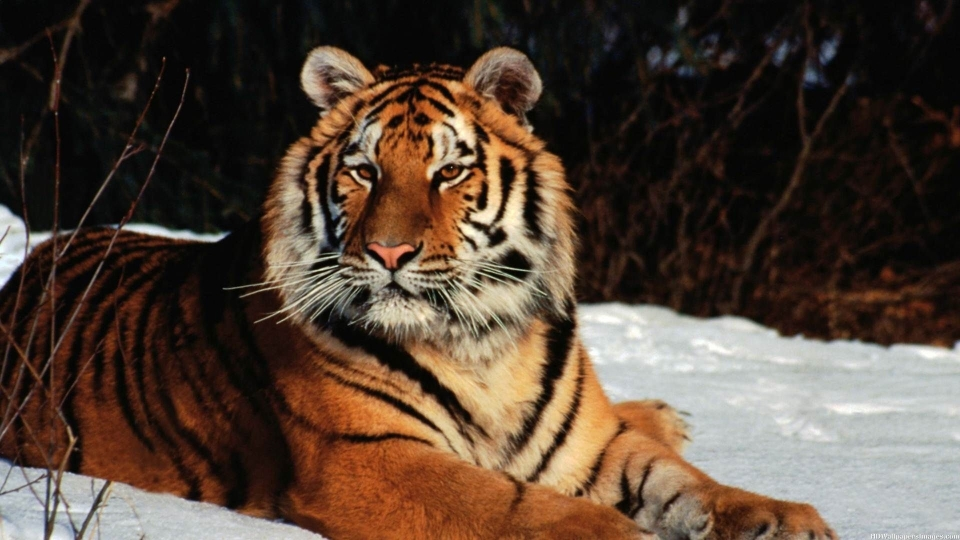
\includegraphics[width=\textwidth]{figures/tiger}
            \caption{Tiger image}
    \end{subfigure}
    \begin{subfigure}[b]{0.33\textwidth}
            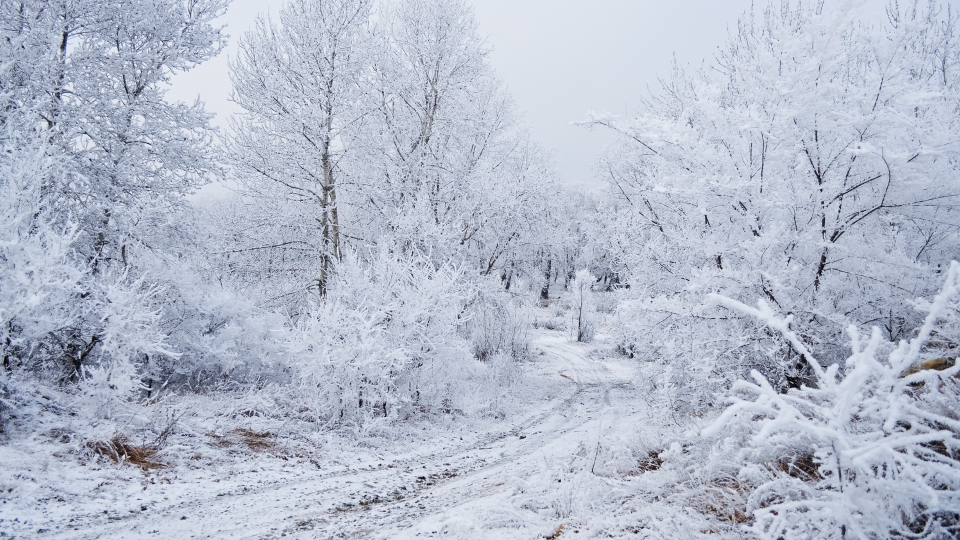
\includegraphics[width=\textwidth]{figures/snow}
            \caption{Snow image}
    \end{subfigure}
    \caption{The four images used for the tests in table \ref{fig:forces_swaps}}
    \label{fig:four_test_images}
\end{figure}

\begin{table}[H]
    \centering
    \resizebox{0.7\textwidth}{!}{%
        \begin{tabular}{@{}lllll@{}}
            \textbf{Image}                      & \textbf{Message length} & \textbf{Swaps} & \textbf{Forces} & \textbf{Already fit} \\ \midrule
            \multirow{5}{*}{\textit{Cat}}       & 70                      & 56\%           & 19\%            & 26\%                 \\
                                                & 140                     & 58\%           & 18\%            & 24\%                 \\
                                                & 280                     & 65\%           & 12\%            & 23\%                 \\
                                                & 560                     & 65\%           & 11\%            & 24\%                 \\
                                                & 1120                    & 66\%           & 8\%             & 25\%                 \\ \midrule
            \multirow{5}{*}{\textit{Landscape}} & 70                      & 55\%           & 15\%            & 30\%                 \\
                                                & 140                     & 63\%           & 11\%            & 27\%                 \\
                                                & 280                     & 62\%           & 11\%            & 27\%                 \\
                                                & 560                     & 62\%           & 13\%            & 25\%                 \\
                                                & 1120                    & 63\%           & 12\%            & 25\%                 \\ \midrule
            \multirow{5}{*}{\textit{Tiger}}     & 70                      & 63\%           & 8\%             & 28\%                 \\
                                                & 140                     & 64\%           & 8\%             & 27\%                 \\
                                                & 280                     & 68\%           & 6\%             & 26\%                 \\
                                                & 560                     & 70\%           & 5\%             & 25\%                 \\
                                                & 1120                    & 72\%           & 4\%             & 24\%                 \\ \midrule
            \multirow{5}{*}{\textit{Snow}}      & 70                      & 53\%           & 21\%            & 26\%                 \\
                                                & 140                     & 58\%           & 13\%            & 29\%                 \\
                                                & 280                     & 66\%           & 8\%             & 26\%                 \\
                                                & 560                     & 67\%           & 8\%             & 25\%                 \\
                                                & 1120                    & 69\%           & 7\%             & 24\%                 \\ \bottomrule
        \end{tabular}
    }
    \caption{The percentages of values which the program swapped or forced. Since this was run with M = 4, about a fourth of the values already fit.}
    \label{fig:forces_swaps}
\end{table}

\subsection{Size of the graph}
It became apparent that a longer message required fewer forces. 
This made sense, seeing as a longer message meant a larger graph with more edges and therefore possible ways of swapping values.
During development of the programme we played around with the idea of using more vertices than what was required for the message, as we predicted it would mean fewer forces.
These predictions would seem to be correct, but we never implemented the idea for two reasons.

One, we were not entirely certain how to do it: should we just use twice as much as was actually needed?
This would lead to using much more than what was necessary with a longer message, since the improvement quickly diminishes with longer messages.
Instead it would make more sense to always use a certain minimum of values, so shorter messages could be encoded properly, but longer ones did not take too long to encode.
What were to happen if the image simply did not contain enough values then? 
Should the programme inform the user that they needed to use a larger image or attempt to encode the message with the vertices it could make?
What would this mean for the \lstinline|GetCapacity| method? 
Should it take into consideration these extra values or just ignore it entirely?
An entirely different approach would be to let the user decide themselves, how many values they wished the algorithm to use. 
Presenting this in a user-friendly way constituted a challenge in itself though.

The second reason we did not implement it was due to performance concerns.
Since our programme performed rather poorly during most of the development we considered it a very bad idea to construct a larger graph than we already were constructing.
Seeing as we managed to optimise the programme quite significantly, we could have properly implemented a solution regardless.

\subsection{Colour histograms}
Actually comparing colour histograms from the two methods was not as trivial as one could have hoped.
Using the LSB-method only made immediately visible changes to the colour histograms if about a quarter of the image had data encoded in it.
When using an image of substantial size, a quarter of an image can hold a large amount of data. 
A 512x512 image for example can hold 196,604 bytes, when using the two least significant bits.
Encoding 40,000 bytes using our graph-theoretical (GT) programme was completely out of the question due to the complexity of the algorithm.
The longest message we tried encoding was just under 8960 bytes and took around half an hour on a decent desktop computer.
Running several test runs with different message lengths made it clear that the complexity of the programme made it impossible to ever complete an encoding of this much data.

This made a direct comparison using realistic real-world images and messages impossible. 
The only real comparison we could make was between images containing different messages that used up every single available byte in the image.
Since the GT method became very time consuming with larger messages, we would need to use an image that was small enough that we could embed all bytes possible, without it taking too long to complete.
We ended up using an image with a resolution of 120x120 pixels.

\begin{figure}
    \centering
    \begin{subfigure}[b]{0.49\textwidth}
        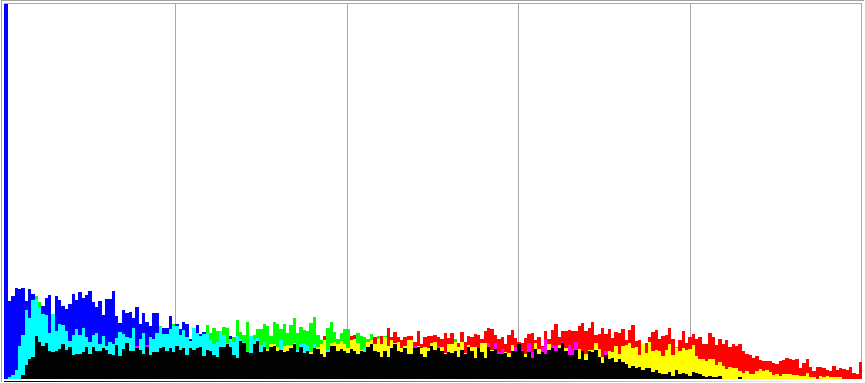
\includegraphics[width=\textwidth]{figures/tiger_smallHisto.png}
            \caption{Cover image}
            \label{fig:coverHisto}
    \end{subfigure}
    \begin{subfigure}[b]{0.49\textwidth}
            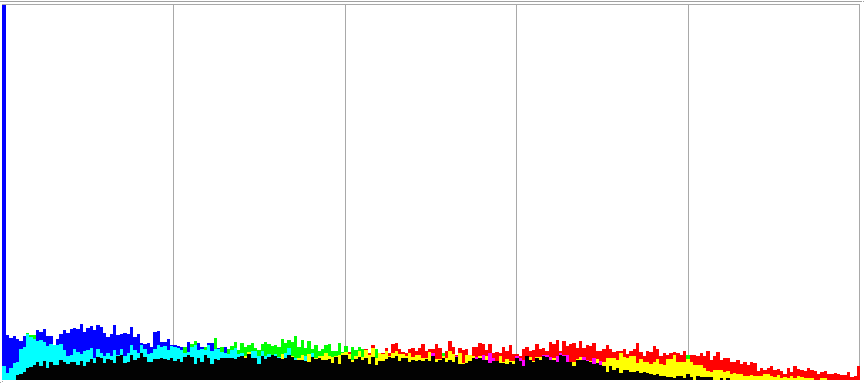
\includegraphics[width=\textwidth]{figures/gtOut2Histo.png}
            \caption{Cover image as JPEG}
            \label{fig:gt2Histo}
    \end{subfigure}
    \begin{subfigure}[b]{0.49\textwidth}
            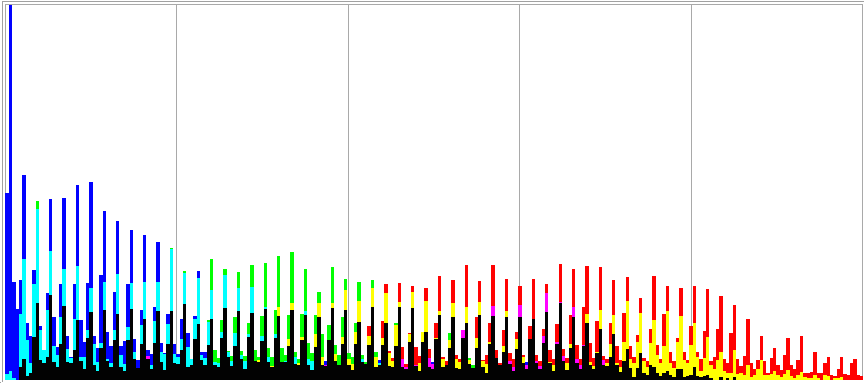
\includegraphics[width=\textwidth]{figures/lsbOutHisto.png}
            \caption{Stego image with message (LSB)}
            \label{fig:lsbHisto}
    \end{subfigure}
    \begin{subfigure}[b]{0.49\textwidth}
            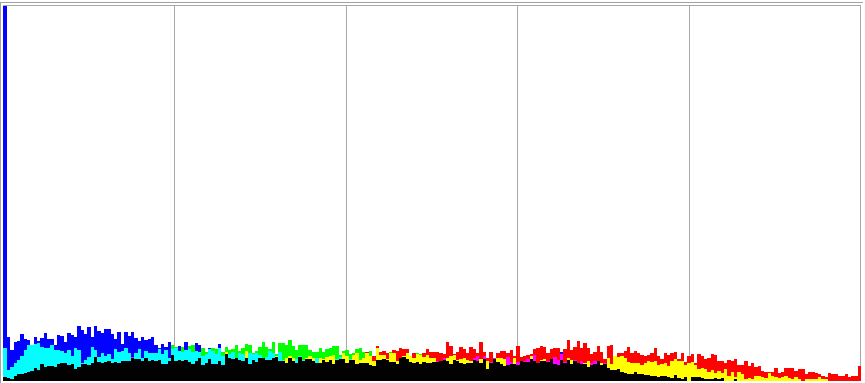
\includegraphics[width=\textwidth]{figures/gtOutHisto.png}
            \caption{Stego image with message (GT)}
            \label{fig:gtHisto}
    \end{subfigure}
    \caption{Histogram of a 120x120 px image}
    \label{fig:histogramsComparisons}
\end{figure}

In figure \ref{fig:histogramsComparisons} four histograms are shown.
Figures \ref{fig:coverHisto} and \ref{fig:gt2Histo} show the histogram of the original image and for the image encoded as JPEG without a message.
In figure \ref{fig:lsbHisto} and \ref{fig:gtHisto} the histograms of the images filled with a message using the LSB and GT methods respectively.
From these results it was clear that there was not much difference between the colour histograms of the image saved as JPEG with or without the message.
The image saved with LSB's histogram, however, clearly showed signs that the image had been tampered with.

The reason the histogram looked like that for the LSB image was because the bit-patterns of the encoded data became very clear in the histograms.
The bytes encoded in the images were the characters A-Z in ASCII repeated the capacity of the image had been reached.
A-Z in ASCII ranges from $65-90$, or in base two: $01000001_2-01011010_2$.
As the range was quite short, a lot of the higher order bits would rarely change, and those patterns became obvious in the histogram, as pixels ending in these patterns became more common.

The histogram in figure \ref{fig:lsbHisto} also showed how the LSB method changed images where a colour is very common.
The leftmost bar described pixels whose B-component is 0.
In the original cover image, this bar was much higher than the others, and therefore much more common in the image, but the LSB has made it so that those components now get spread out, which again becomes very obvious in the histogram.

\subsection{Euclidean distance}
A different way of looking for changes in an image is by looking at their Euclidean distance.
This can be done by calculating the distance between the colour values of each pixel in two equally sized images.
The sum of all these distances can be used as measure of the change from one image to the other.
We used this same method for determining what changes were imposed on images of different size and format, when uploaded to various social media and image-sharing websites.
The images used for the method were the same as those previously used in the colour histogram tests.
The results of these tests can be seen in table \ref {fig:euclidean_distance}.

\begin{table}[]
	\centering
	\begin{tabular}{@{}lllll@{}}
		\toprule
		\textbf{Images}            & \textbf{All channels} & \textbf{R} & \textbf{G} & \textbf{B} \\ \midrule
		\textit{Original and LSB}  & 34671                 & 17098      & 16800      & 16824      \\
		\textit{Original and GT}   & 130389                & 71112      & 56972      & 71886      \\
		\textit{Original and JPEG} & 102460                & 56758      & 40707      & 57569      \\
		\textit{JPEG and GT}       & 79163                 & 42154      & 38833      & 43217     
	\end{tabular}
	\caption{Calculated euclidean distances for several combinations of images.}
	\label{fig:euclidean_distance}
\end{table}


Comparing these results directly with the ones obtained from the LSB-method would be folly.
While the LSB-method might incur a smaller difference in the Euclidean distance it would not necessarily make it any better.

The other reason for the differences being larger is due to how the JPEG-file format is encoded.
Using the LSB of every pixel there is only the potential to change the value of each pixel by one.
Using the graph-theoretical approach with an M value of four, means that each individual value can be changed by four. 
This change is applied after the quantization step to avoid losing the data again.
This in turn means that the small change of up to four is multiplied by the quantization table, when the image is shown.
Bla bla something something green is less than the other

First of all using this method required that the user was in possession of both the original and the stego image.
This would indeed be possible if the parties sharing secret messages in the images, were using images they found on the internet and tampered with them.
Ths meant that they could completely foil any risk of being compromised by an outside party measuring euclidean distance, by simply using images that they took themselves.

So while the Euclidean distance might be bigger in the image where the data is hidden using our GT programme, it is of little use in automated system doing steganalysis on a multitude of images, as it would have nothing to compare the images to. 
Such a system could however check the histogram of the image, and discover abnormalities such as those the LSB method produces, as shown in figure \ref{fig:lsbHisto}.
	
\chapter{Conclusion}\label{ch:conclusion}

	\section{Introduction to Steganography}
Through the ages, people have been dependent on efficient forms of communication. In some cases, these messages would include information that should ideally be confidential and not read by anyone else other than the intended recipient. To do this, would require a way of concealing the details of the message in a way that an outsider would not be able to decipher what the actual message is.

Whereas cryptography is about concealing a message's content in a way that reveals that a message is concealed(which would undoubtedly raise some form of suspicion), steganography is about concealing the message's existence. This means that instead of the private message's content being protected by an obvious security-measure, people have had to find ways of circumventing interception and hide their messages in plain view to avoid any suspicion. This is one advantage steganography has over cryptography. 

Steganography is the art of concealing a message in a cover object, without having other people being aware that the concealed message is being sent.\cite{Anderson1998} The cover object could be in the form of video, audio or plain text. An example of this could be, hiding information in something innocuous that is not likely to get any unwanted, extra attention. The concealment should be subtle, so that unless a person was aware there was something to be found, is very unlikely to notice that a message is being passed in front of them without their notice.

As not everyone wishes to have every detail of their life, scrutinised and under the watch of everyone, people have had to implement forms of steganography to get their meaning across to their intended recipient. This goes back centuries, for example, people in ancient China would write messages on fine silk, which would then be pressed together until it was a much smaller piece of material and covered in wax. The cover of this message, was a person who would have to swallow the message to bring the information safely, without interception to the intended receiver. \cite{Singh2001} Another example being medieval Europe, where they had a system using templates, which would then be placed over a text, highlighting what the actual message is.\cite{Anderson1998}

Since then, forms of steganography have become much more advanced, and naturally, digitalised. Steganography can be implemented by anyone, no matter their intention, but would most typically be people who feel like they have something to hide. With the rise of social media, sending messages via the internet, and specifically these social media networks, has become the norm. Therefore it is only natural that a modern form of steganography should be able to work on these platforms. 

	% -*- root: ../../DAT2-A423_Project_Report.tex -*-
\section{Discussion}
We started out by using the relatively simple LSB-method for hiding data in an image.
Specifically, we saved an image inside of another PNG-image.
While the differences in the image with and without the message-image were hardly noticeable to the human eye, we did find that comparing colour histograms of the two images revealed that there had in fact been made changes to it.
In an effort to diminish this problem, the graph-theoretical approach we implemented attempted to move pixels around in the image, rather than change their values.
This meant that colour histograms of the image before and after the message had been encoded should look very similar, almost identical.
Any changes would come from the unmatched pairs: the quantized DCT values used in the encoding that we did not find any interchangeable values for.
When this happened we were forced to change the individual values, which led to a change in the colour composition of the image.
Using this method, we expected the changes to be small enough so that it would not immediately draw attention to the image, if it was being subjected to a colour histogram.

\subsection{Changes to the image}
To find out roughly how many of these forces there were in a given image, we used our programme to save different messages in different images.
The used five different message lengths were: 70, 140, 280, 560 and 1120 bytes.
Each message consisted of the ASCII characters A-Z repeated to fill out the message.
Each of these messages were encoded in four images with varying motives, but the same resolution (1920x1080).
The images can be seen in figure \ref{fig:four_test_images}.

We used a cartoon-like drawing of a cat to see how our software would work on an image that was not ideal for the JPEG format.
The landscape image contained many different colours and very complex patterns, which made it ideal for JPEG compression.
The same could be said for the tiger, but it contained larger areas of similar colours than the landscape did.
The image of the snowy forest road contained very few colour nuances, but was almost entirely made up of the luminance channel.
This led to a total of 20 tests as seen in table \ref{fig:forces_swaps}.

\begin{figure}[H]
    \centering
    \begin{subfigure}[b]{0.33\textwidth}
        
\includegraphics[width=\textwidth]{figures/cat}
            \caption{Cat image}
    \end{subfigure}
    \begin{subfigure}[b]{0.33\textwidth}
            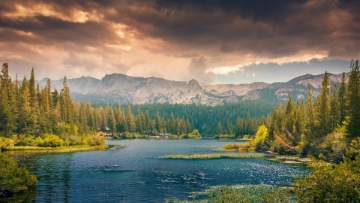
\includegraphics[width=\textwidth]{figures/landscape}
            \caption{Landscape image}
    \end{subfigure}
    \begin{subfigure}[b]{0.33\textwidth}
            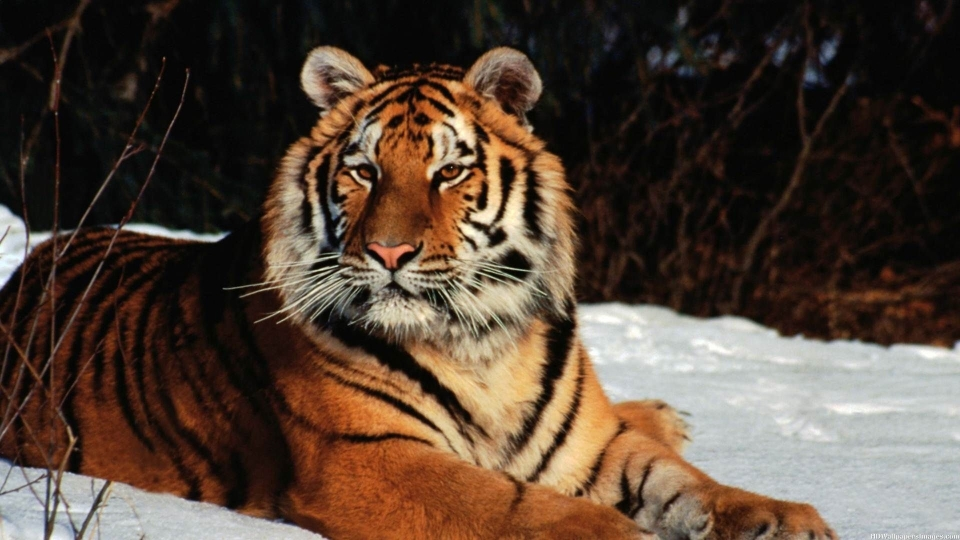
\includegraphics[width=\textwidth]{figures/tiger}
            \caption{Tiger image}
    \end{subfigure}
    \begin{subfigure}[b]{0.33\textwidth}
            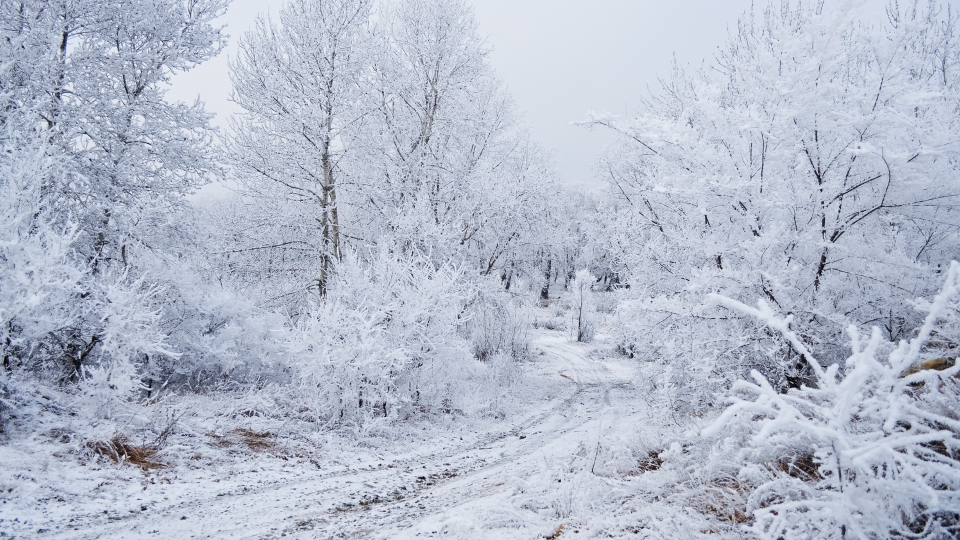
\includegraphics[width=\textwidth]{figures/snow}
            \caption{Snow image}
    \end{subfigure}
    \caption{The four images used for the tests in table \ref{fig:forces_swaps}}
    \label{fig:four_test_images}
\end{figure}

\begin{table}[H]
    \centering
    \resizebox{0.7\textwidth}{!}{%
        \begin{tabular}{@{}lllll@{}}
            \textbf{Image}                      & \textbf{Message length} & \textbf{Swaps} & \textbf{Forces} & \textbf{Already fit} \\ \midrule
            \multirow{5}{*}{\textit{Cat}}       & 70                      & 56\%           & 19\%            & 26\%                 \\
                                                & 140                     & 58\%           & 18\%            & 24\%                 \\
                                                & 280                     & 65\%           & 12\%            & 23\%                 \\
                                                & 560                     & 65\%           & 11\%            & 24\%                 \\
                                                & 1120                    & 66\%           & 8\%             & 25\%                 \\ \midrule
            \multirow{5}{*}{\textit{Landscape}} & 70                      & 55\%           & 15\%            & 30\%                 \\
                                                & 140                     & 63\%           & 11\%            & 27\%                 \\
                                                & 280                     & 62\%           & 11\%            & 27\%                 \\
                                                & 560                     & 62\%           & 13\%            & 25\%                 \\
                                                & 1120                    & 63\%           & 12\%            & 25\%                 \\ \midrule
            \multirow{5}{*}{\textit{Tiger}}     & 70                      & 63\%           & 8\%             & 28\%                 \\
                                                & 140                     & 64\%           & 8\%             & 27\%                 \\
                                                & 280                     & 68\%           & 6\%             & 26\%                 \\
                                                & 560                     & 70\%           & 5\%             & 25\%                 \\
                                                & 1120                    & 72\%           & 4\%             & 24\%                 \\ \midrule
            \multirow{5}{*}{\textit{Snow}}      & 70                      & 53\%           & 21\%            & 26\%                 \\
                                                & 140                     & 58\%           & 13\%            & 29\%                 \\
                                                & 280                     & 66\%           & 8\%             & 26\%                 \\
                                                & 560                     & 67\%           & 8\%             & 25\%                 \\
                                                & 1120                    & 69\%           & 7\%             & 24\%                 \\ \bottomrule
        \end{tabular}
    }
    \caption{The percentages of values which the program swapped or forced. Since this was run with M = 4, about a fourth of the values already fit.}
    \label{fig:forces_swaps}
\end{table}

\subsection{Size of the graph}
It became apparent that a longer message required fewer forces. 
This made sense, seeing as a longer message meant a larger graph with more edges and therefore possible ways of swapping values.
During development of the programme we played around with the idea of using more vertices than what was required for the message, as we predicted it would mean fewer forces.
These predictions would seem to be correct, but we never implemented the idea for two reasons.

One, we were not entirely certain how to do it: should we just use twice as much as was actually needed?
This would lead to using much more than what was necessary with a longer message, since the improvement quickly diminishes with longer messages.
Instead it would make more sense to always use a certain minimum of values, so shorter messages could be encoded properly, but longer ones did not take too long to encode.
What were to happen if the image simply did not contain enough values then? 
Should the programme inform the user that they needed to use a larger image or attempt to encode the message with the vertices it could make?
What would this mean for the \lstinline|GetCapacity| method? 
Should it take into consideration these extra values or just ignore it entirely?
An entirely different approach would be to let the user decide themselves, how many values they wished the algorithm to use. 
Presenting this in a user-friendly way constituted a challenge in itself though.

The second reason we did not implement it was due to performance concerns.
Since our programme performed rather poorly during most of the development we considered it a very bad idea to construct a larger graph than we already were constructing.
Seeing as we managed to optimise the programme quite significantly, we could have properly implemented a solution regardless.

\subsection{Colour histograms}
Actually comparing colour histograms from the two methods was not as trivial as one could have hoped.
Using the LSB-method only made immediately visible changes to the colour histograms if about a quarter of the image had data encoded in it.
When using an image of substantial size, a quarter of an image can hold a large amount of data. 
A 512x512 image for example can hold 196,604 bytes, when using the two least significant bits.
Encoding 40,000 bytes using our graph-theoretical (GT) programme was completely out of the question due to the complexity of the algorithm.
The longest message we tried encoding was just under 8960 bytes and took around half an hour on a decent desktop computer.
Running several test runs with different message lengths made it clear that the complexity of the programme made it impossible to ever complete an encoding of this much data.

This made a direct comparison using realistic real-world images and messages impossible. 
The only real comparison we could make was between images containing different messages that used up every single available byte in the image.
Since the GT method became very time consuming with larger messages, we would need to use an image that was small enough that we could embed all bytes possible, without it taking too long to complete.
We ended up using an image with a resolution of 120x120 pixels.

\begin{figure}
    \centering
    \begin{subfigure}[b]{0.49\textwidth}
        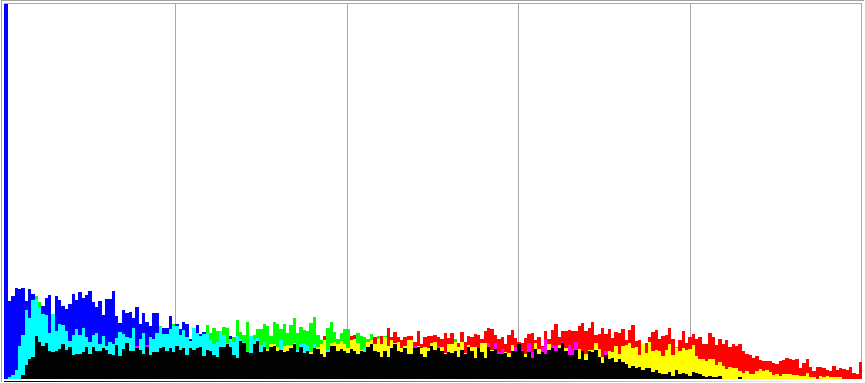
\includegraphics[width=\textwidth]{figures/tiger_smallHisto.png}
            \caption{Cover image}
            \label{fig:coverHisto}
    \end{subfigure}
    \begin{subfigure}[b]{0.49\textwidth}
            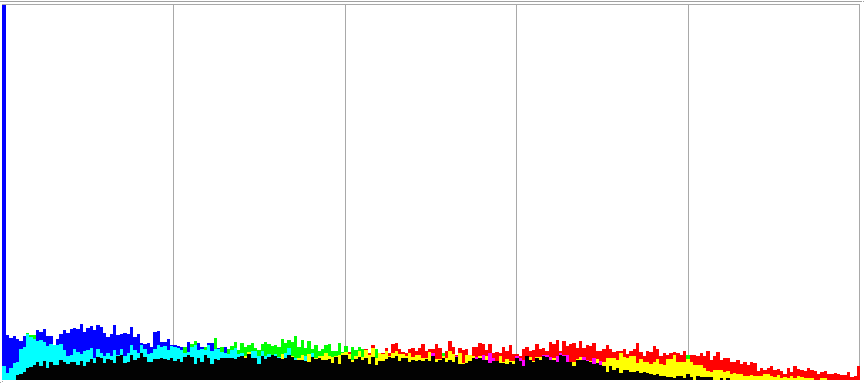
\includegraphics[width=\textwidth]{figures/gtOut2Histo.png}
            \caption{Cover image as JPEG}
            \label{fig:gt2Histo}
    \end{subfigure}
    \begin{subfigure}[b]{0.49\textwidth}
            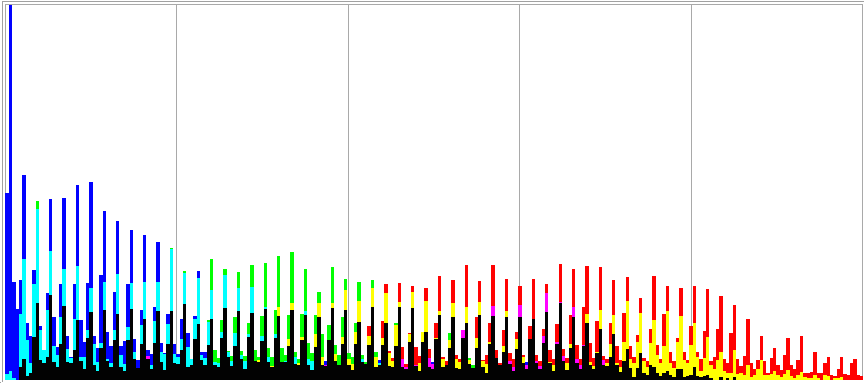
\includegraphics[width=\textwidth]{figures/lsbOutHisto.png}
            \caption{Stego image with message (LSB)}
            \label{fig:lsbHisto}
    \end{subfigure}
    \begin{subfigure}[b]{0.49\textwidth}
            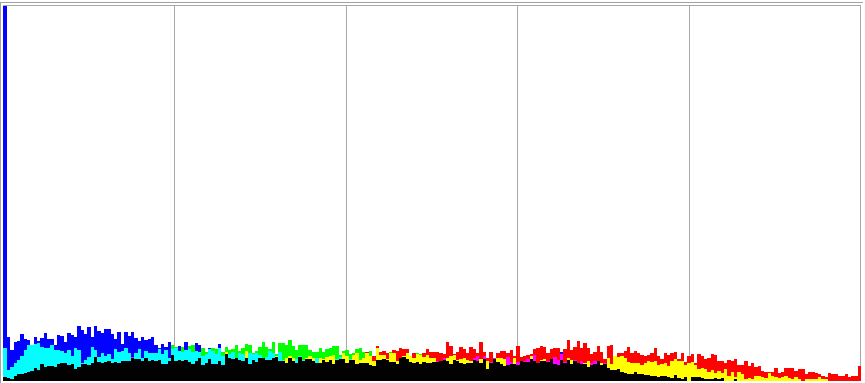
\includegraphics[width=\textwidth]{figures/gtOutHisto.png}
            \caption{Stego image with message (GT)}
            \label{fig:gtHisto}
    \end{subfigure}
    \caption{Histogram of a 120x120 px image}
    \label{fig:histogramsComparisons}
\end{figure}

In figure \ref{fig:histogramsComparisons} four histograms are shown.
Figures \ref{fig:coverHisto} and \ref{fig:gt2Histo} show the histogram of the original image and for the image encoded as JPEG without a message.
In figure \ref{fig:lsbHisto} and \ref{fig:gtHisto} the histograms of the images filled with a message using the LSB and GT methods respectively.
From these results it was clear that there was not much difference between the colour histograms of the image saved as JPEG with or without the message.
The image saved with LSB's histogram, however, clearly showed signs that the image had been tampered with.

The reason the histogram looked like that for the LSB image was because the bit-patterns of the encoded data became very clear in the histograms.
The bytes encoded in the images were the characters A-Z in ASCII repeated the capacity of the image had been reached.
A-Z in ASCII ranges from $65-90$, or in base two: $01000001_2-01011010_2$.
As the range was quite short, a lot of the higher order bits would rarely change, and those patterns became obvious in the histogram, as pixels ending in these patterns became more common.

The histogram in figure \ref{fig:lsbHisto} also showed how the LSB method changed images where a colour is very common.
The leftmost bar described pixels whose B-component is 0.
In the original cover image, this bar was much higher than the others, and therefore much more common in the image, but the LSB has made it so that those components now get spread out, which again becomes very obvious in the histogram.

\subsection{Euclidean distance}
A different way of looking for changes in an image is by looking at their Euclidean distance.
This can be done by calculating the distance between the colour values of each pixel in two equally sized images.
The sum of all these distances can be used as measure of the change from one image to the other.
We used this same method for determining what changes were imposed on images of different size and format, when uploaded to various social media and image-sharing websites.
The images used for the method were the same as those previously used in the colour histogram tests.
The results of these tests can be seen in table \ref {fig:euclidean_distance}.

\begin{table}[]
	\centering
	\begin{tabular}{@{}lllll@{}}
		\toprule
		\textbf{Images}            & \textbf{All channels} & \textbf{R} & \textbf{G} & \textbf{B} \\ \midrule
		\textit{Original and LSB}  & 34671                 & 17098      & 16800      & 16824      \\
		\textit{Original and GT}   & 130389                & 71112      & 56972      & 71886      \\
		\textit{Original and JPEG} & 102460                & 56758      & 40707      & 57569      \\
		\textit{JPEG and GT}       & 79163                 & 42154      & 38833      & 43217     
	\end{tabular}
	\caption{Calculated euclidean distances for several combinations of images.}
	\label{fig:euclidean_distance}
\end{table}


Comparing these results directly with the ones obtained from the LSB-method would be folly.
While the LSB-method might incur a smaller difference in the Euclidean distance it would not necessarily make it any better.

The other reason for the differences being larger is due to how the JPEG-file format is encoded.
Using the LSB of every pixel there is only the potential to change the value of each pixel by one.
Using the graph-theoretical approach with an M value of four, means that each individual value can be changed by four. 
This change is applied after the quantization step to avoid losing the data again.
This in turn means that the small change of up to four is multiplied by the quantization table, when the image is shown.
Bla bla something something green is less than the other

First of all using this method required that the user was in possession of both the original and the stego image.
This would indeed be possible if the parties sharing secret messages in the images, were using images they found on the internet and tampered with them.
Ths meant that they could completely foil any risk of being compromised by an outside party measuring euclidean distance, by simply using images that they took themselves.

So while the Euclidean distance might be bigger in the image where the data is hidden using our GT programme, it is of little use in automated system doing steganalysis on a multitude of images, as it would have nothing to compare the images to. 
Such a system could however check the histogram of the image, and discover abnormalities such as those the LSB method produces, as shown in figure \ref{fig:lsbHisto}.
	
%\chapter{Conclusion}\label{ch:conclusion}

	\section{Introduction to Steganography}
Through the ages, people have been dependent on efficient forms of communication. In some cases, these messages would include information that should ideally be confidential and not read by anyone else other than the intended recipient. To do this, would require a way of concealing the details of the message in a way that an outsider would not be able to decipher what the actual message is.

Whereas cryptography is about concealing a message's content in a way that reveals that a message is concealed(which would undoubtedly raise some form of suspicion), steganography is about concealing the message's existence. This means that instead of the private message's content being protected by an obvious security-measure, people have had to find ways of circumventing interception and hide their messages in plain view to avoid any suspicion. This is one advantage steganography has over cryptography. 

Steganography is the art of concealing a message in a cover object, without having other people being aware that the concealed message is being sent.\cite{Anderson1998} The cover object could be in the form of video, audio or plain text. An example of this could be, hiding information in something innocuous that is not likely to get any unwanted, extra attention. The concealment should be subtle, so that unless a person was aware there was something to be found, is very unlikely to notice that a message is being passed in front of them without their notice.

As not everyone wishes to have every detail of their life, scrutinised and under the watch of everyone, people have had to implement forms of steganography to get their meaning across to their intended recipient. This goes back centuries, for example, people in ancient China would write messages on fine silk, which would then be pressed together until it was a much smaller piece of material and covered in wax. The cover of this message, was a person who would have to swallow the message to bring the information safely, without interception to the intended receiver. \cite{Singh2001} Another example being medieval Europe, where they had a system using templates, which would then be placed over a text, highlighting what the actual message is.\cite{Anderson1998}

Since then, forms of steganography have become much more advanced, and naturally, digitalised. Steganography can be implemented by anyone, no matter their intention, but would most typically be people who feel like they have something to hide. With the rise of social media, sending messages via the internet, and specifically these social media networks, has become the norm. Therefore it is only natural that a modern form of steganography should be able to work on these platforms. 

	% -*- root: ../../DAT2-A423_Project_Report.tex -*-
\section{Discussion}
We started out by using the relatively simple LSB-method for hiding data in an image.
Specifically, we saved an image inside of another PNG-image.
While the differences in the image with and without the message-image were hardly noticeable to the human eye, we did find that comparing colour histograms of the two images revealed that there had in fact been made changes to it.
In an effort to diminish this problem, the graph-theoretical approach we implemented attempted to move pixels around in the image, rather than change their values.
This meant that colour histograms of the image before and after the message had been encoded should look very similar, almost identical.
Any changes would come from the unmatched pairs: the quantized DCT values used in the encoding that we did not find any interchangeable values for.
When this happened we were forced to change the individual values, which led to a change in the colour composition of the image.
Using this method, we expected the changes to be small enough so that it would not immediately draw attention to the image, if it was being subjected to a colour histogram.

\subsection{Changes to the image}
To find out roughly how many of these forces there were in a given image, we used our programme to save different messages in different images.
The used five different message lengths were: 70, 140, 280, 560 and 1120 bytes.
Each message consisted of the ASCII characters A-Z repeated to fill out the message.
Each of these messages were encoded in four images with varying motives, but the same resolution (1920x1080).
The images can be seen in figure \ref{fig:four_test_images}.

We used a cartoon-like drawing of a cat to see how our software would work on an image that was not ideal for the JPEG format.
The landscape image contained many different colours and very complex patterns, which made it ideal for JPEG compression.
The same could be said for the tiger, but it contained larger areas of similar colours than the landscape did.
The image of the snowy forest road contained very few colour nuances, but was almost entirely made up of the luminance channel.
This led to a total of 20 tests as seen in table \ref{fig:forces_swaps}.

\begin{figure}[H]
    \centering
    \begin{subfigure}[b]{0.33\textwidth}
        
\includegraphics[width=\textwidth]{figures/cat}
            \caption{Cat image}
    \end{subfigure}
    \begin{subfigure}[b]{0.33\textwidth}
            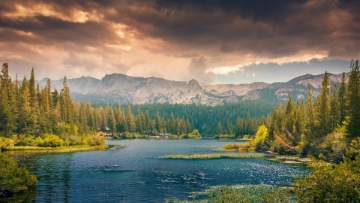
\includegraphics[width=\textwidth]{figures/landscape}
            \caption{Landscape image}
    \end{subfigure}
    \begin{subfigure}[b]{0.33\textwidth}
            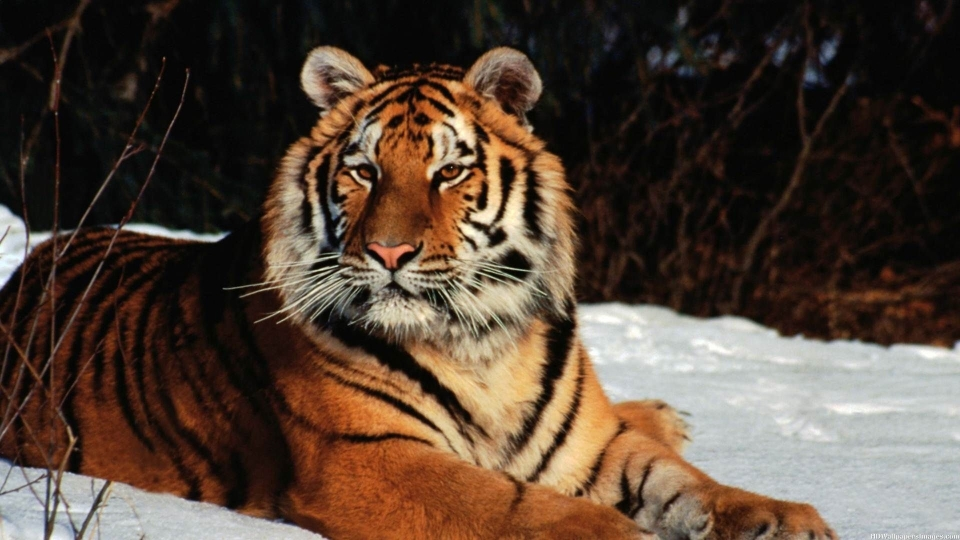
\includegraphics[width=\textwidth]{figures/tiger}
            \caption{Tiger image}
    \end{subfigure}
    \begin{subfigure}[b]{0.33\textwidth}
            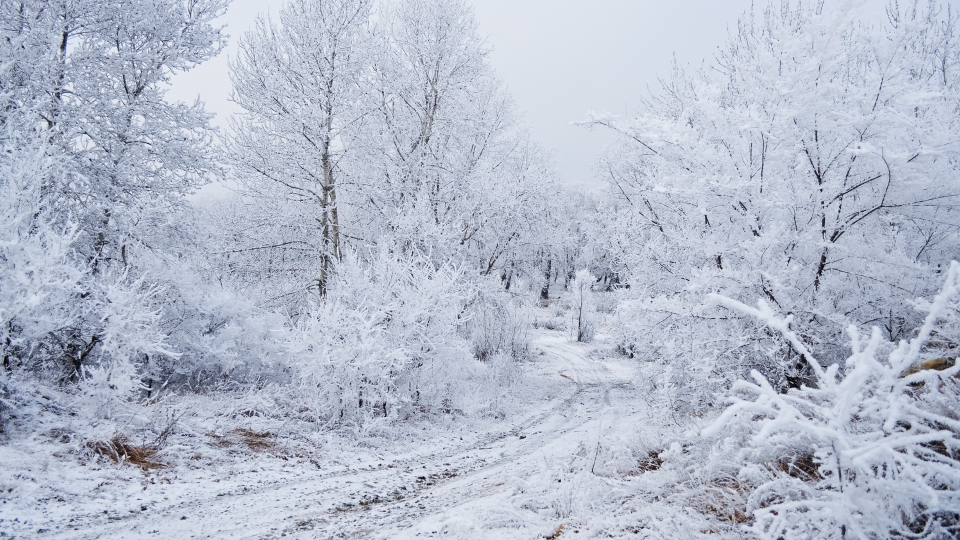
\includegraphics[width=\textwidth]{figures/snow}
            \caption{Snow image}
    \end{subfigure}
    \caption{The four images used for the tests in table \ref{fig:forces_swaps}}
    \label{fig:four_test_images}
\end{figure}

\begin{table}[H]
    \centering
    \resizebox{0.7\textwidth}{!}{%
        \begin{tabular}{@{}lllll@{}}
            \textbf{Image}                      & \textbf{Message length} & \textbf{Swaps} & \textbf{Forces} & \textbf{Already fit} \\ \midrule
            \multirow{5}{*}{\textit{Cat}}       & 70                      & 56\%           & 19\%            & 26\%                 \\
                                                & 140                     & 58\%           & 18\%            & 24\%                 \\
                                                & 280                     & 65\%           & 12\%            & 23\%                 \\
                                                & 560                     & 65\%           & 11\%            & 24\%                 \\
                                                & 1120                    & 66\%           & 8\%             & 25\%                 \\ \midrule
            \multirow{5}{*}{\textit{Landscape}} & 70                      & 55\%           & 15\%            & 30\%                 \\
                                                & 140                     & 63\%           & 11\%            & 27\%                 \\
                                                & 280                     & 62\%           & 11\%            & 27\%                 \\
                                                & 560                     & 62\%           & 13\%            & 25\%                 \\
                                                & 1120                    & 63\%           & 12\%            & 25\%                 \\ \midrule
            \multirow{5}{*}{\textit{Tiger}}     & 70                      & 63\%           & 8\%             & 28\%                 \\
                                                & 140                     & 64\%           & 8\%             & 27\%                 \\
                                                & 280                     & 68\%           & 6\%             & 26\%                 \\
                                                & 560                     & 70\%           & 5\%             & 25\%                 \\
                                                & 1120                    & 72\%           & 4\%             & 24\%                 \\ \midrule
            \multirow{5}{*}{\textit{Snow}}      & 70                      & 53\%           & 21\%            & 26\%                 \\
                                                & 140                     & 58\%           & 13\%            & 29\%                 \\
                                                & 280                     & 66\%           & 8\%             & 26\%                 \\
                                                & 560                     & 67\%           & 8\%             & 25\%                 \\
                                                & 1120                    & 69\%           & 7\%             & 24\%                 \\ \bottomrule
        \end{tabular}
    }
    \caption{The percentages of values which the program swapped or forced. Since this was run with M = 4, about a fourth of the values already fit.}
    \label{fig:forces_swaps}
\end{table}

\subsection{Size of the graph}
It became apparent that a longer message required fewer forces. 
This made sense, seeing as a longer message meant a larger graph with more edges and therefore possible ways of swapping values.
During development of the programme we played around with the idea of using more vertices than what was required for the message, as we predicted it would mean fewer forces.
These predictions would seem to be correct, but we never implemented the idea for two reasons.

One, we were not entirely certain how to do it: should we just use twice as much as was actually needed?
This would lead to using much more than what was necessary with a longer message, since the improvement quickly diminishes with longer messages.
Instead it would make more sense to always use a certain minimum of values, so shorter messages could be encoded properly, but longer ones did not take too long to encode.
What were to happen if the image simply did not contain enough values then? 
Should the programme inform the user that they needed to use a larger image or attempt to encode the message with the vertices it could make?
What would this mean for the \lstinline|GetCapacity| method? 
Should it take into consideration these extra values or just ignore it entirely?
An entirely different approach would be to let the user decide themselves, how many values they wished the algorithm to use. 
Presenting this in a user-friendly way constituted a challenge in itself though.

The second reason we did not implement it was due to performance concerns.
Since our programme performed rather poorly during most of the development we considered it a very bad idea to construct a larger graph than we already were constructing.
Seeing as we managed to optimise the programme quite significantly, we could have properly implemented a solution regardless.

\subsection{Colour histograms}
Actually comparing colour histograms from the two methods was not as trivial as one could have hoped.
Using the LSB-method only made immediately visible changes to the colour histograms if about a quarter of the image had data encoded in it.
When using an image of substantial size, a quarter of an image can hold a large amount of data. 
A 512x512 image for example can hold 196,604 bytes, when using the two least significant bits.
Encoding 40,000 bytes using our graph-theoretical (GT) programme was completely out of the question due to the complexity of the algorithm.
The longest message we tried encoding was just under 8960 bytes and took around half an hour on a decent desktop computer.
Running several test runs with different message lengths made it clear that the complexity of the programme made it impossible to ever complete an encoding of this much data.

This made a direct comparison using realistic real-world images and messages impossible. 
The only real comparison we could make was between images containing different messages that used up every single available byte in the image.
Since the GT method became very time consuming with larger messages, we would need to use an image that was small enough that we could embed all bytes possible, without it taking too long to complete.
We ended up using an image with a resolution of 120x120 pixels.

\begin{figure}
    \centering
    \begin{subfigure}[b]{0.49\textwidth}
        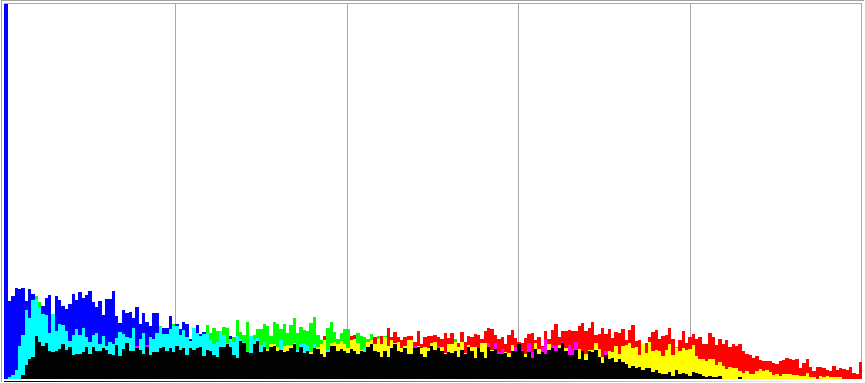
\includegraphics[width=\textwidth]{figures/tiger_smallHisto.png}
            \caption{Cover image}
            \label{fig:coverHisto}
    \end{subfigure}
    \begin{subfigure}[b]{0.49\textwidth}
            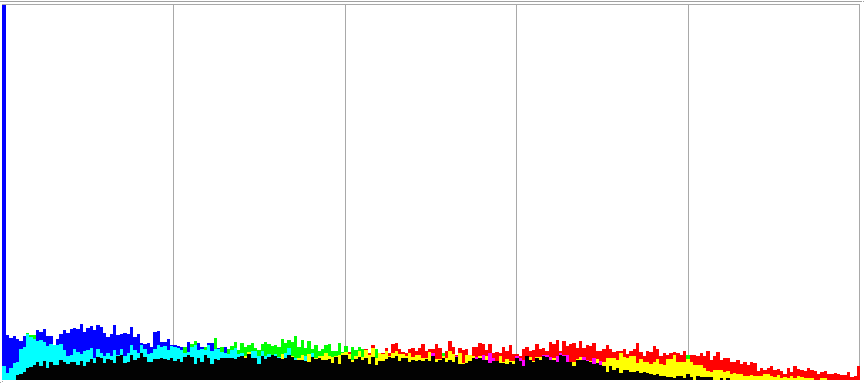
\includegraphics[width=\textwidth]{figures/gtOut2Histo.png}
            \caption{Cover image as JPEG}
            \label{fig:gt2Histo}
    \end{subfigure}
    \begin{subfigure}[b]{0.49\textwidth}
            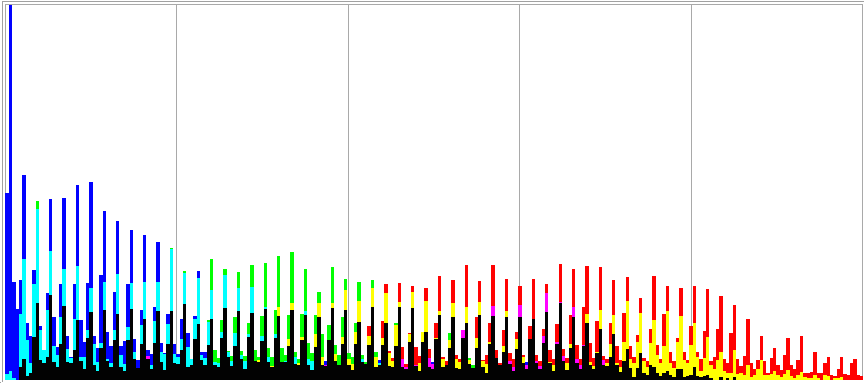
\includegraphics[width=\textwidth]{figures/lsbOutHisto.png}
            \caption{Stego image with message (LSB)}
            \label{fig:lsbHisto}
    \end{subfigure}
    \begin{subfigure}[b]{0.49\textwidth}
            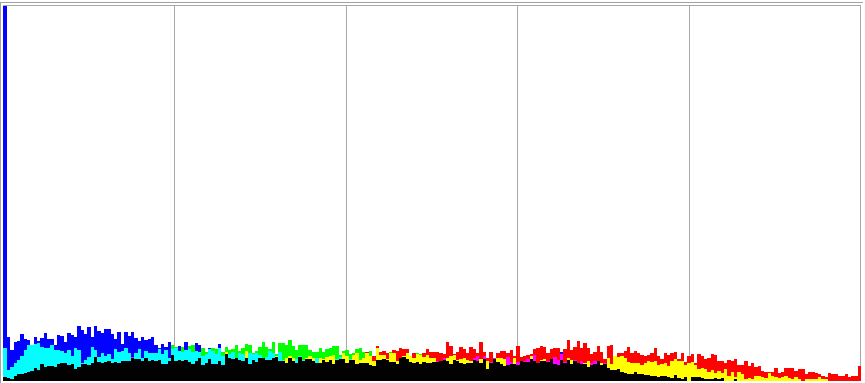
\includegraphics[width=\textwidth]{figures/gtOutHisto.png}
            \caption{Stego image with message (GT)}
            \label{fig:gtHisto}
    \end{subfigure}
    \caption{Histogram of a 120x120 px image}
    \label{fig:histogramsComparisons}
\end{figure}

In figure \ref{fig:histogramsComparisons} four histograms are shown.
Figures \ref{fig:coverHisto} and \ref{fig:gt2Histo} show the histogram of the original image and for the image encoded as JPEG without a message.
In figure \ref{fig:lsbHisto} and \ref{fig:gtHisto} the histograms of the images filled with a message using the LSB and GT methods respectively.
From these results it was clear that there was not much difference between the colour histograms of the image saved as JPEG with or without the message.
The image saved with LSB's histogram, however, clearly showed signs that the image had been tampered with.

The reason the histogram looked like that for the LSB image was because the bit-patterns of the encoded data became very clear in the histograms.
The bytes encoded in the images were the characters A-Z in ASCII repeated the capacity of the image had been reached.
A-Z in ASCII ranges from $65-90$, or in base two: $01000001_2-01011010_2$.
As the range was quite short, a lot of the higher order bits would rarely change, and those patterns became obvious in the histogram, as pixels ending in these patterns became more common.

The histogram in figure \ref{fig:lsbHisto} also showed how the LSB method changed images where a colour is very common.
The leftmost bar described pixels whose B-component is 0.
In the original cover image, this bar was much higher than the others, and therefore much more common in the image, but the LSB has made it so that those components now get spread out, which again becomes very obvious in the histogram.

\subsection{Euclidean distance}
A different way of looking for changes in an image is by looking at their Euclidean distance.
This can be done by calculating the distance between the colour values of each pixel in two equally sized images.
The sum of all these distances can be used as measure of the change from one image to the other.
We used this same method for determining what changes were imposed on images of different size and format, when uploaded to various social media and image-sharing websites.
The images used for the method were the same as those previously used in the colour histogram tests.
The results of these tests can be seen in table \ref {fig:euclidean_distance}.

\begin{table}[]
	\centering
	\begin{tabular}{@{}lllll@{}}
		\toprule
		\textbf{Images}            & \textbf{All channels} & \textbf{R} & \textbf{G} & \textbf{B} \\ \midrule
		\textit{Original and LSB}  & 34671                 & 17098      & 16800      & 16824      \\
		\textit{Original and GT}   & 130389                & 71112      & 56972      & 71886      \\
		\textit{Original and JPEG} & 102460                & 56758      & 40707      & 57569      \\
		\textit{JPEG and GT}       & 79163                 & 42154      & 38833      & 43217     
	\end{tabular}
	\caption{Calculated euclidean distances for several combinations of images.}
	\label{fig:euclidean_distance}
\end{table}


Comparing these results directly with the ones obtained from the LSB-method would be folly.
While the LSB-method might incur a smaller difference in the Euclidean distance it would not necessarily make it any better.

The other reason for the differences being larger is due to how the JPEG-file format is encoded.
Using the LSB of every pixel there is only the potential to change the value of each pixel by one.
Using the graph-theoretical approach with an M value of four, means that each individual value can be changed by four. 
This change is applied after the quantization step to avoid losing the data again.
This in turn means that the small change of up to four is multiplied by the quantization table, when the image is shown.
Bla bla something something green is less than the other

First of all using this method required that the user was in possession of both the original and the stego image.
This would indeed be possible if the parties sharing secret messages in the images, were using images they found on the internet and tampered with them.
Ths meant that they could completely foil any risk of being compromised by an outside party measuring euclidean distance, by simply using images that they took themselves.

So while the Euclidean distance might be bigger in the image where the data is hidden using our GT programme, it is of little use in automated system doing steganalysis on a multitude of images, as it would have nothing to compare the images to. 
Such a system could however check the histogram of the image, and discover abnormalities such as those the LSB method produces, as shown in figure \ref{fig:lsbHisto}.
	
%\chapter{Conclusion}\label{ch:conclusion}

	\section{Introduction to Steganography}
Through the ages, people have been dependent on efficient forms of communication. In some cases, these messages would include information that should ideally be confidential and not read by anyone else other than the intended recipient. To do this, would require a way of concealing the details of the message in a way that an outsider would not be able to decipher what the actual message is.

Whereas cryptography is about concealing a message's content in a way that reveals that a message is concealed(which would undoubtedly raise some form of suspicion), steganography is about concealing the message's existence. This means that instead of the private message's content being protected by an obvious security-measure, people have had to find ways of circumventing interception and hide their messages in plain view to avoid any suspicion. This is one advantage steganography has over cryptography. 

Steganography is the art of concealing a message in a cover object, without having other people being aware that the concealed message is being sent.\cite{Anderson1998} The cover object could be in the form of video, audio or plain text. An example of this could be, hiding information in something innocuous that is not likely to get any unwanted, extra attention. The concealment should be subtle, so that unless a person was aware there was something to be found, is very unlikely to notice that a message is being passed in front of them without their notice.

As not everyone wishes to have every detail of their life, scrutinised and under the watch of everyone, people have had to implement forms of steganography to get their meaning across to their intended recipient. This goes back centuries, for example, people in ancient China would write messages on fine silk, which would then be pressed together until it was a much smaller piece of material and covered in wax. The cover of this message, was a person who would have to swallow the message to bring the information safely, without interception to the intended receiver. \cite{Singh2001} Another example being medieval Europe, where they had a system using templates, which would then be placed over a text, highlighting what the actual message is.\cite{Anderson1998}

Since then, forms of steganography have become much more advanced, and naturally, digitalised. Steganography can be implemented by anyone, no matter their intention, but would most typically be people who feel like they have something to hide. With the rise of social media, sending messages via the internet, and specifically these social media networks, has become the norm. Therefore it is only natural that a modern form of steganography should be able to work on these platforms. 

	% -*- root: ../../DAT2-A423_Project_Report.tex -*-
\section{Discussion}
We started out by using the relatively simple LSB-method for hiding data in an image.
Specifically, we saved an image inside of another PNG-image.
While the differences in the image with and without the message-image were hardly noticeable to the human eye, we did find that comparing colour histograms of the two images revealed that there had in fact been made changes to it.
In an effort to diminish this problem, the graph-theoretical approach we implemented attempted to move pixels around in the image, rather than change their values.
This meant that colour histograms of the image before and after the message had been encoded should look very similar, almost identical.
Any changes would come from the unmatched pairs: the quantized DCT values used in the encoding that we did not find any interchangeable values for.
When this happened we were forced to change the individual values, which led to a change in the colour composition of the image.
Using this method, we expected the changes to be small enough so that it would not immediately draw attention to the image, if it was being subjected to a colour histogram.

\subsection{Changes to the image}
To find out roughly how many of these forces there were in a given image, we used our programme to save different messages in different images.
The used five different message lengths were: 70, 140, 280, 560 and 1120 bytes.
Each message consisted of the ASCII characters A-Z repeated to fill out the message.
Each of these messages were encoded in four images with varying motives, but the same resolution (1920x1080).
The images can be seen in figure \ref{fig:four_test_images}.

We used a cartoon-like drawing of a cat to see how our software would work on an image that was not ideal for the JPEG format.
The landscape image contained many different colours and very complex patterns, which made it ideal for JPEG compression.
The same could be said for the tiger, but it contained larger areas of similar colours than the landscape did.
The image of the snowy forest road contained very few colour nuances, but was almost entirely made up of the luminance channel.
This led to a total of 20 tests as seen in table \ref{fig:forces_swaps}.

\begin{figure}[H]
    \centering
    \begin{subfigure}[b]{0.33\textwidth}
        
\includegraphics[width=\textwidth]{figures/cat}
            \caption{Cat image}
    \end{subfigure}
    \begin{subfigure}[b]{0.33\textwidth}
            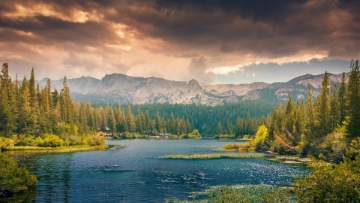
\includegraphics[width=\textwidth]{figures/landscape}
            \caption{Landscape image}
    \end{subfigure}
    \begin{subfigure}[b]{0.33\textwidth}
            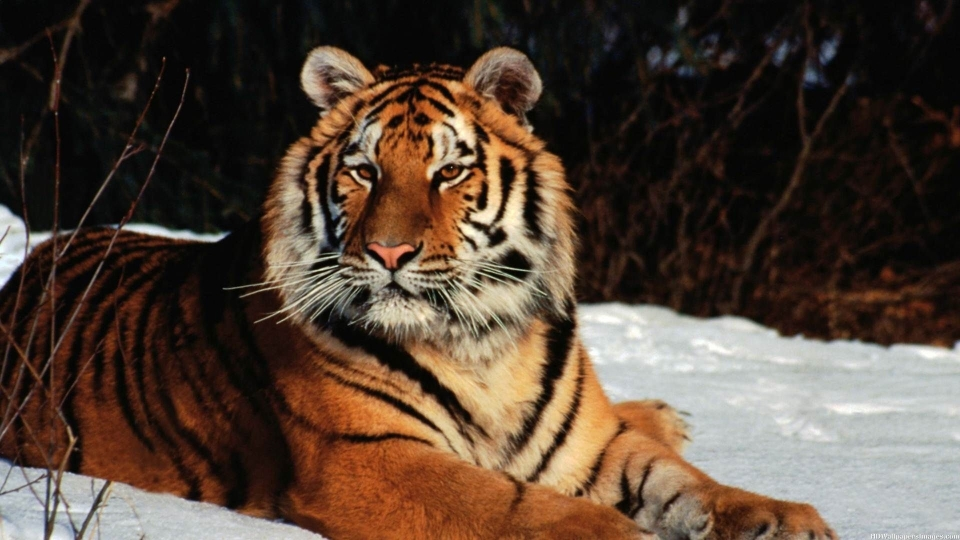
\includegraphics[width=\textwidth]{figures/tiger}
            \caption{Tiger image}
    \end{subfigure}
    \begin{subfigure}[b]{0.33\textwidth}
            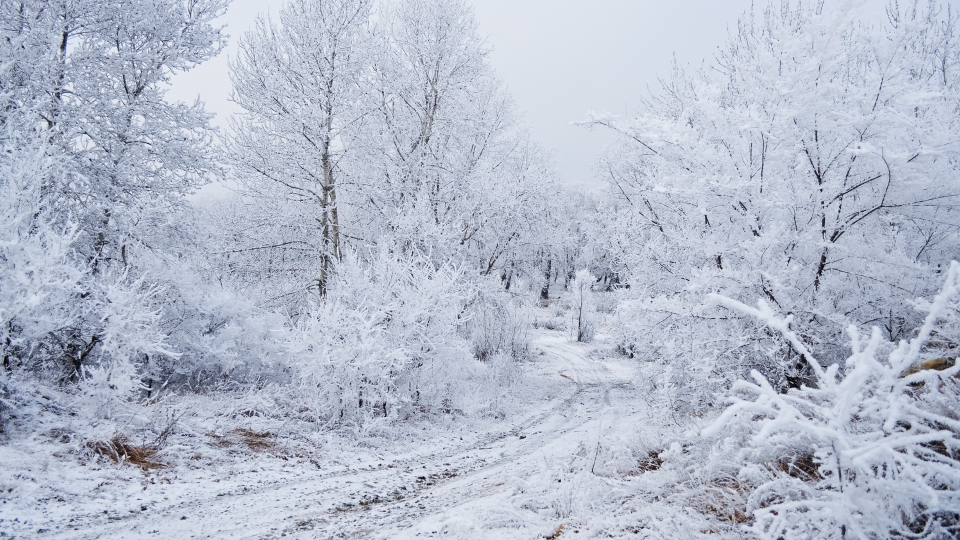
\includegraphics[width=\textwidth]{figures/snow}
            \caption{Snow image}
    \end{subfigure}
    \caption{The four images used for the tests in table \ref{fig:forces_swaps}}
    \label{fig:four_test_images}
\end{figure}

\begin{table}[H]
    \centering
    \resizebox{0.7\textwidth}{!}{%
        \begin{tabular}{@{}lllll@{}}
            \textbf{Image}                      & \textbf{Message length} & \textbf{Swaps} & \textbf{Forces} & \textbf{Already fit} \\ \midrule
            \multirow{5}{*}{\textit{Cat}}       & 70                      & 56\%           & 19\%            & 26\%                 \\
                                                & 140                     & 58\%           & 18\%            & 24\%                 \\
                                                & 280                     & 65\%           & 12\%            & 23\%                 \\
                                                & 560                     & 65\%           & 11\%            & 24\%                 \\
                                                & 1120                    & 66\%           & 8\%             & 25\%                 \\ \midrule
            \multirow{5}{*}{\textit{Landscape}} & 70                      & 55\%           & 15\%            & 30\%                 \\
                                                & 140                     & 63\%           & 11\%            & 27\%                 \\
                                                & 280                     & 62\%           & 11\%            & 27\%                 \\
                                                & 560                     & 62\%           & 13\%            & 25\%                 \\
                                                & 1120                    & 63\%           & 12\%            & 25\%                 \\ \midrule
            \multirow{5}{*}{\textit{Tiger}}     & 70                      & 63\%           & 8\%             & 28\%                 \\
                                                & 140                     & 64\%           & 8\%             & 27\%                 \\
                                                & 280                     & 68\%           & 6\%             & 26\%                 \\
                                                & 560                     & 70\%           & 5\%             & 25\%                 \\
                                                & 1120                    & 72\%           & 4\%             & 24\%                 \\ \midrule
            \multirow{5}{*}{\textit{Snow}}      & 70                      & 53\%           & 21\%            & 26\%                 \\
                                                & 140                     & 58\%           & 13\%            & 29\%                 \\
                                                & 280                     & 66\%           & 8\%             & 26\%                 \\
                                                & 560                     & 67\%           & 8\%             & 25\%                 \\
                                                & 1120                    & 69\%           & 7\%             & 24\%                 \\ \bottomrule
        \end{tabular}
    }
    \caption{The percentages of values which the program swapped or forced. Since this was run with M = 4, about a fourth of the values already fit.}
    \label{fig:forces_swaps}
\end{table}

\subsection{Size of the graph}
It became apparent that a longer message required fewer forces. 
This made sense, seeing as a longer message meant a larger graph with more edges and therefore possible ways of swapping values.
During development of the programme we played around with the idea of using more vertices than what was required for the message, as we predicted it would mean fewer forces.
These predictions would seem to be correct, but we never implemented the idea for two reasons.

One, we were not entirely certain how to do it: should we just use twice as much as was actually needed?
This would lead to using much more than what was necessary with a longer message, since the improvement quickly diminishes with longer messages.
Instead it would make more sense to always use a certain minimum of values, so shorter messages could be encoded properly, but longer ones did not take too long to encode.
What were to happen if the image simply did not contain enough values then? 
Should the programme inform the user that they needed to use a larger image or attempt to encode the message with the vertices it could make?
What would this mean for the \lstinline|GetCapacity| method? 
Should it take into consideration these extra values or just ignore it entirely?
An entirely different approach would be to let the user decide themselves, how many values they wished the algorithm to use. 
Presenting this in a user-friendly way constituted a challenge in itself though.

The second reason we did not implement it was due to performance concerns.
Since our programme performed rather poorly during most of the development we considered it a very bad idea to construct a larger graph than we already were constructing.
Seeing as we managed to optimise the programme quite significantly, we could have properly implemented a solution regardless.

\subsection{Colour histograms}
Actually comparing colour histograms from the two methods was not as trivial as one could have hoped.
Using the LSB-method only made immediately visible changes to the colour histograms if about a quarter of the image had data encoded in it.
When using an image of substantial size, a quarter of an image can hold a large amount of data. 
A 512x512 image for example can hold 196,604 bytes, when using the two least significant bits.
Encoding 40,000 bytes using our graph-theoretical (GT) programme was completely out of the question due to the complexity of the algorithm.
The longest message we tried encoding was just under 8960 bytes and took around half an hour on a decent desktop computer.
Running several test runs with different message lengths made it clear that the complexity of the programme made it impossible to ever complete an encoding of this much data.

This made a direct comparison using realistic real-world images and messages impossible. 
The only real comparison we could make was between images containing different messages that used up every single available byte in the image.
Since the GT method became very time consuming with larger messages, we would need to use an image that was small enough that we could embed all bytes possible, without it taking too long to complete.
We ended up using an image with a resolution of 120x120 pixels.

\begin{figure}
    \centering
    \begin{subfigure}[b]{0.49\textwidth}
        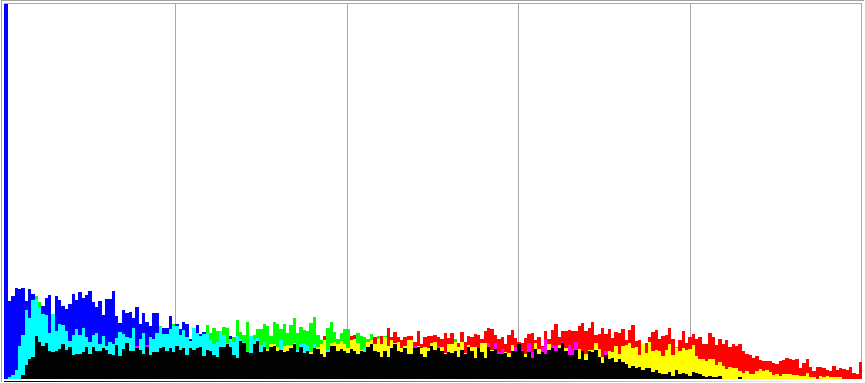
\includegraphics[width=\textwidth]{figures/tiger_smallHisto.png}
            \caption{Cover image}
            \label{fig:coverHisto}
    \end{subfigure}
    \begin{subfigure}[b]{0.49\textwidth}
            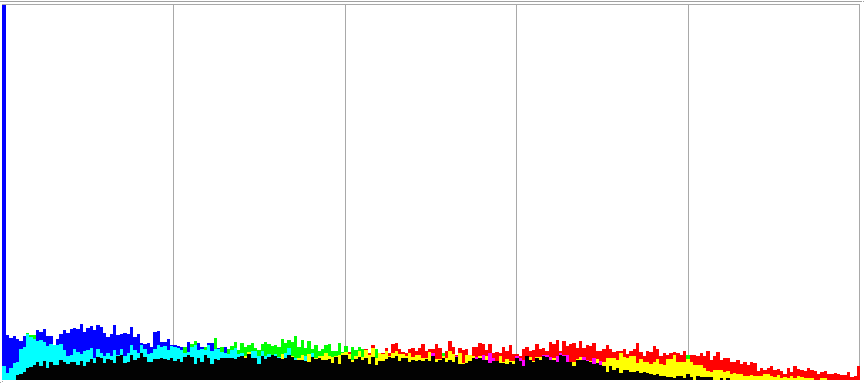
\includegraphics[width=\textwidth]{figures/gtOut2Histo.png}
            \caption{Cover image as JPEG}
            \label{fig:gt2Histo}
    \end{subfigure}
    \begin{subfigure}[b]{0.49\textwidth}
            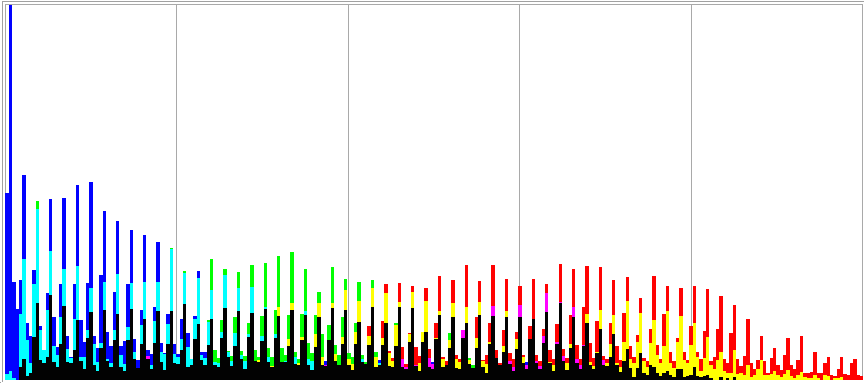
\includegraphics[width=\textwidth]{figures/lsbOutHisto.png}
            \caption{Stego image with message (LSB)}
            \label{fig:lsbHisto}
    \end{subfigure}
    \begin{subfigure}[b]{0.49\textwidth}
            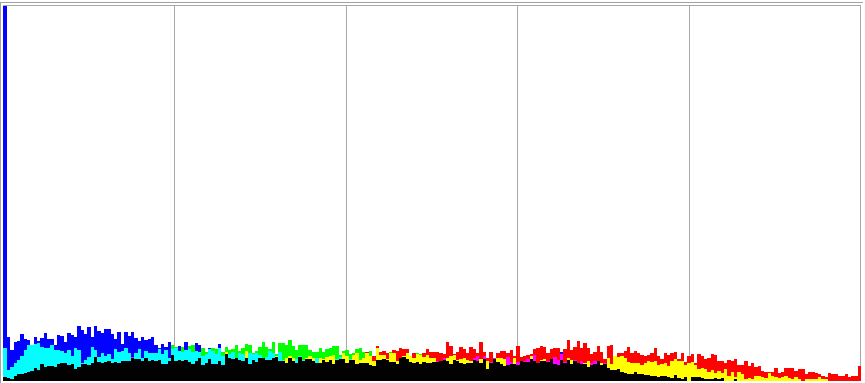
\includegraphics[width=\textwidth]{figures/gtOutHisto.png}
            \caption{Stego image with message (GT)}
            \label{fig:gtHisto}
    \end{subfigure}
    \caption{Histogram of a 120x120 px image}
    \label{fig:histogramsComparisons}
\end{figure}

In figure \ref{fig:histogramsComparisons} four histograms are shown.
Figures \ref{fig:coverHisto} and \ref{fig:gt2Histo} show the histogram of the original image and for the image encoded as JPEG without a message.
In figure \ref{fig:lsbHisto} and \ref{fig:gtHisto} the histograms of the images filled with a message using the LSB and GT methods respectively.
From these results it was clear that there was not much difference between the colour histograms of the image saved as JPEG with or without the message.
The image saved with LSB's histogram, however, clearly showed signs that the image had been tampered with.

The reason the histogram looked like that for the LSB image was because the bit-patterns of the encoded data became very clear in the histograms.
The bytes encoded in the images were the characters A-Z in ASCII repeated the capacity of the image had been reached.
A-Z in ASCII ranges from $65-90$, or in base two: $01000001_2-01011010_2$.
As the range was quite short, a lot of the higher order bits would rarely change, and those patterns became obvious in the histogram, as pixels ending in these patterns became more common.

The histogram in figure \ref{fig:lsbHisto} also showed how the LSB method changed images where a colour is very common.
The leftmost bar described pixels whose B-component is 0.
In the original cover image, this bar was much higher than the others, and therefore much more common in the image, but the LSB has made it so that those components now get spread out, which again becomes very obvious in the histogram.

\subsection{Euclidean distance}
A different way of looking for changes in an image is by looking at their Euclidean distance.
This can be done by calculating the distance between the colour values of each pixel in two equally sized images.
The sum of all these distances can be used as measure of the change from one image to the other.
We used this same method for determining what changes were imposed on images of different size and format, when uploaded to various social media and image-sharing websites.
The images used for the method were the same as those previously used in the colour histogram tests.
The results of these tests can be seen in table \ref {fig:euclidean_distance}.

\begin{table}[]
	\centering
	\begin{tabular}{@{}lllll@{}}
		\toprule
		\textbf{Images}            & \textbf{All channels} & \textbf{R} & \textbf{G} & \textbf{B} \\ \midrule
		\textit{Original and LSB}  & 34671                 & 17098      & 16800      & 16824      \\
		\textit{Original and GT}   & 130389                & 71112      & 56972      & 71886      \\
		\textit{Original and JPEG} & 102460                & 56758      & 40707      & 57569      \\
		\textit{JPEG and GT}       & 79163                 & 42154      & 38833      & 43217     
	\end{tabular}
	\caption{Calculated euclidean distances for several combinations of images.}
	\label{fig:euclidean_distance}
\end{table}


Comparing these results directly with the ones obtained from the LSB-method would be folly.
While the LSB-method might incur a smaller difference in the Euclidean distance it would not necessarily make it any better.

The other reason for the differences being larger is due to how the JPEG-file format is encoded.
Using the LSB of every pixel there is only the potential to change the value of each pixel by one.
Using the graph-theoretical approach with an M value of four, means that each individual value can be changed by four. 
This change is applied after the quantization step to avoid losing the data again.
This in turn means that the small change of up to four is multiplied by the quantization table, when the image is shown.
Bla bla something something green is less than the other

First of all using this method required that the user was in possession of both the original and the stego image.
This would indeed be possible if the parties sharing secret messages in the images, were using images they found on the internet and tampered with them.
Ths meant that they could completely foil any risk of being compromised by an outside party measuring euclidean distance, by simply using images that they took themselves.

So while the Euclidean distance might be bigger in the image where the data is hidden using our GT programme, it is of little use in automated system doing steganalysis on a multitude of images, as it would have nothing to compare the images to. 
Such a system could however check the histogram of the image, and discover abnormalities such as those the LSB method produces, as shown in figure \ref{fig:lsbHisto}.
	
%\chapter{Conclusion}\label{ch:conclusion}

	\section{Introduction to Steganography}
Through the ages, people have been dependent on efficient forms of communication. In some cases, these messages would include information that should ideally be confidential and not read by anyone else other than the intended recipient. To do this, would require a way of concealing the details of the message in a way that an outsider would not be able to decipher what the actual message is.

Whereas cryptography is about concealing a message's content in a way that reveals that a message is concealed(which would undoubtedly raise some form of suspicion), steganography is about concealing the message's existence. This means that instead of the private message's content being protected by an obvious security-measure, people have had to find ways of circumventing interception and hide their messages in plain view to avoid any suspicion. This is one advantage steganography has over cryptography. 

Steganography is the art of concealing a message in a cover object, without having other people being aware that the concealed message is being sent.\cite{Anderson1998} The cover object could be in the form of video, audio or plain text. An example of this could be, hiding information in something innocuous that is not likely to get any unwanted, extra attention. The concealment should be subtle, so that unless a person was aware there was something to be found, is very unlikely to notice that a message is being passed in front of them without their notice.

As not everyone wishes to have every detail of their life, scrutinised and under the watch of everyone, people have had to implement forms of steganography to get their meaning across to their intended recipient. This goes back centuries, for example, people in ancient China would write messages on fine silk, which would then be pressed together until it was a much smaller piece of material and covered in wax. The cover of this message, was a person who would have to swallow the message to bring the information safely, without interception to the intended receiver. \cite{Singh2001} Another example being medieval Europe, where they had a system using templates, which would then be placed over a text, highlighting what the actual message is.\cite{Anderson1998}

Since then, forms of steganography have become much more advanced, and naturally, digitalised. Steganography can be implemented by anyone, no matter their intention, but would most typically be people who feel like they have something to hide. With the rise of social media, sending messages via the internet, and specifically these social media networks, has become the norm. Therefore it is only natural that a modern form of steganography should be able to work on these platforms. 

	% -*- root: ../../DAT2-A423_Project_Report.tex -*-
\section{Discussion}
We started out by using the relatively simple LSB-method for hiding data in an image.
Specifically, we saved an image inside of another PNG-image.
While the differences in the image with and without the message-image were hardly noticeable to the human eye, we did find that comparing colour histograms of the two images revealed that there had in fact been made changes to it.
In an effort to diminish this problem, the graph-theoretical approach we implemented attempted to move pixels around in the image, rather than change their values.
This meant that colour histograms of the image before and after the message had been encoded should look very similar, almost identical.
Any changes would come from the unmatched pairs: the quantized DCT values used in the encoding that we did not find any interchangeable values for.
When this happened we were forced to change the individual values, which led to a change in the colour composition of the image.
Using this method, we expected the changes to be small enough so that it would not immediately draw attention to the image, if it was being subjected to a colour histogram.

\subsection{Changes to the image}
To find out roughly how many of these forces there were in a given image, we used our programme to save different messages in different images.
The used five different message lengths were: 70, 140, 280, 560 and 1120 bytes.
Each message consisted of the ASCII characters A-Z repeated to fill out the message.
Each of these messages were encoded in four images with varying motives, but the same resolution (1920x1080).
The images can be seen in figure \ref{fig:four_test_images}.

We used a cartoon-like drawing of a cat to see how our software would work on an image that was not ideal for the JPEG format.
The landscape image contained many different colours and very complex patterns, which made it ideal for JPEG compression.
The same could be said for the tiger, but it contained larger areas of similar colours than the landscape did.
The image of the snowy forest road contained very few colour nuances, but was almost entirely made up of the luminance channel.
This led to a total of 20 tests as seen in table \ref{fig:forces_swaps}.

\begin{figure}[H]
    \centering
    \begin{subfigure}[b]{0.33\textwidth}
        
\includegraphics[width=\textwidth]{figures/cat}
            \caption{Cat image}
    \end{subfigure}
    \begin{subfigure}[b]{0.33\textwidth}
            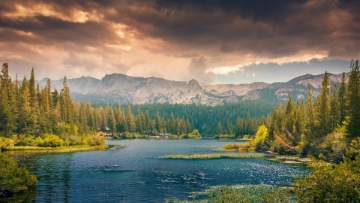
\includegraphics[width=\textwidth]{figures/landscape}
            \caption{Landscape image}
    \end{subfigure}
    \begin{subfigure}[b]{0.33\textwidth}
            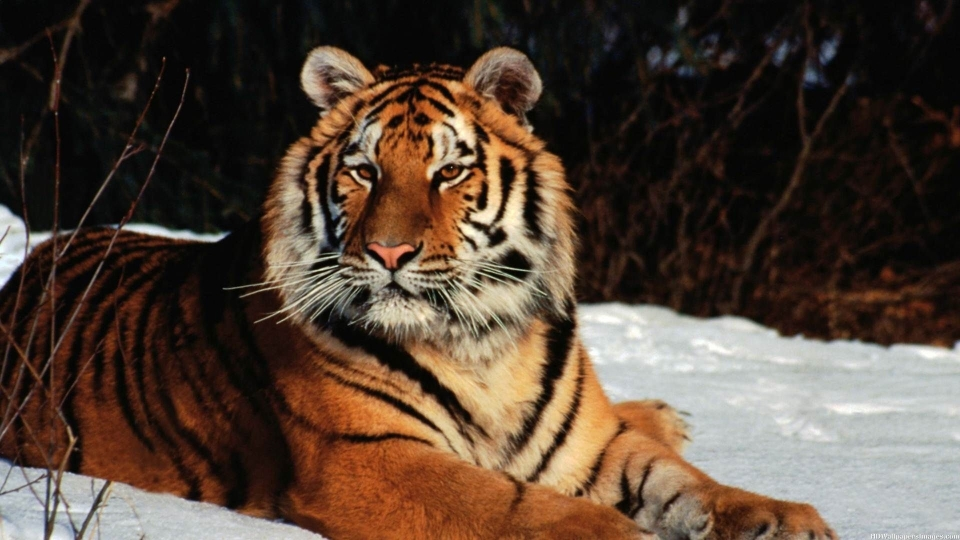
\includegraphics[width=\textwidth]{figures/tiger}
            \caption{Tiger image}
    \end{subfigure}
    \begin{subfigure}[b]{0.33\textwidth}
            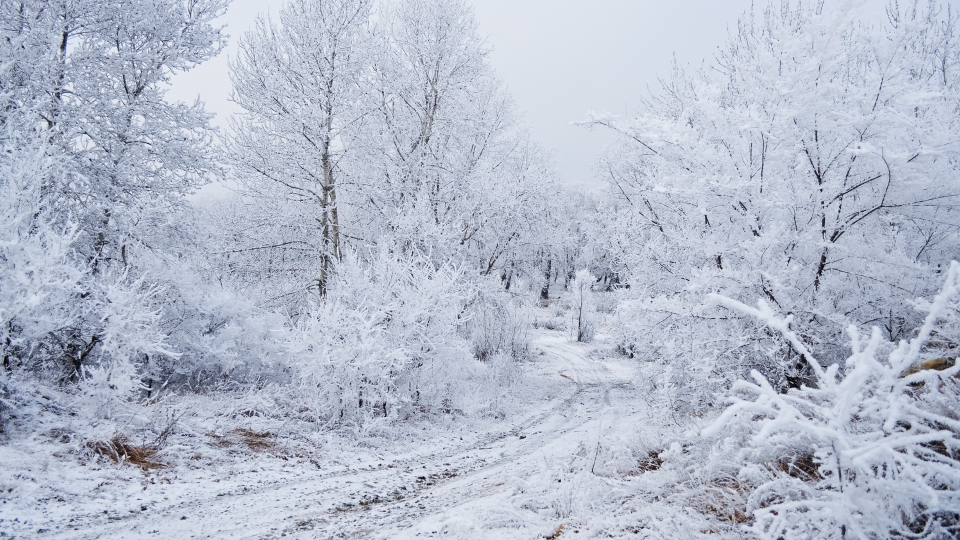
\includegraphics[width=\textwidth]{figures/snow}
            \caption{Snow image}
    \end{subfigure}
    \caption{The four images used for the tests in table \ref{fig:forces_swaps}}
    \label{fig:four_test_images}
\end{figure}

\begin{table}[H]
    \centering
    \resizebox{0.7\textwidth}{!}{%
        \begin{tabular}{@{}lllll@{}}
            \textbf{Image}                      & \textbf{Message length} & \textbf{Swaps} & \textbf{Forces} & \textbf{Already fit} \\ \midrule
            \multirow{5}{*}{\textit{Cat}}       & 70                      & 56\%           & 19\%            & 26\%                 \\
                                                & 140                     & 58\%           & 18\%            & 24\%                 \\
                                                & 280                     & 65\%           & 12\%            & 23\%                 \\
                                                & 560                     & 65\%           & 11\%            & 24\%                 \\
                                                & 1120                    & 66\%           & 8\%             & 25\%                 \\ \midrule
            \multirow{5}{*}{\textit{Landscape}} & 70                      & 55\%           & 15\%            & 30\%                 \\
                                                & 140                     & 63\%           & 11\%            & 27\%                 \\
                                                & 280                     & 62\%           & 11\%            & 27\%                 \\
                                                & 560                     & 62\%           & 13\%            & 25\%                 \\
                                                & 1120                    & 63\%           & 12\%            & 25\%                 \\ \midrule
            \multirow{5}{*}{\textit{Tiger}}     & 70                      & 63\%           & 8\%             & 28\%                 \\
                                                & 140                     & 64\%           & 8\%             & 27\%                 \\
                                                & 280                     & 68\%           & 6\%             & 26\%                 \\
                                                & 560                     & 70\%           & 5\%             & 25\%                 \\
                                                & 1120                    & 72\%           & 4\%             & 24\%                 \\ \midrule
            \multirow{5}{*}{\textit{Snow}}      & 70                      & 53\%           & 21\%            & 26\%                 \\
                                                & 140                     & 58\%           & 13\%            & 29\%                 \\
                                                & 280                     & 66\%           & 8\%             & 26\%                 \\
                                                & 560                     & 67\%           & 8\%             & 25\%                 \\
                                                & 1120                    & 69\%           & 7\%             & 24\%                 \\ \bottomrule
        \end{tabular}
    }
    \caption{The percentages of values which the program swapped or forced. Since this was run with M = 4, about a fourth of the values already fit.}
    \label{fig:forces_swaps}
\end{table}

\subsection{Size of the graph}
It became apparent that a longer message required fewer forces. 
This made sense, seeing as a longer message meant a larger graph with more edges and therefore possible ways of swapping values.
During development of the programme we played around with the idea of using more vertices than what was required for the message, as we predicted it would mean fewer forces.
These predictions would seem to be correct, but we never implemented the idea for two reasons.

One, we were not entirely certain how to do it: should we just use twice as much as was actually needed?
This would lead to using much more than what was necessary with a longer message, since the improvement quickly diminishes with longer messages.
Instead it would make more sense to always use a certain minimum of values, so shorter messages could be encoded properly, but longer ones did not take too long to encode.
What were to happen if the image simply did not contain enough values then? 
Should the programme inform the user that they needed to use a larger image or attempt to encode the message with the vertices it could make?
What would this mean for the \lstinline|GetCapacity| method? 
Should it take into consideration these extra values or just ignore it entirely?
An entirely different approach would be to let the user decide themselves, how many values they wished the algorithm to use. 
Presenting this in a user-friendly way constituted a challenge in itself though.

The second reason we did not implement it was due to performance concerns.
Since our programme performed rather poorly during most of the development we considered it a very bad idea to construct a larger graph than we already were constructing.
Seeing as we managed to optimise the programme quite significantly, we could have properly implemented a solution regardless.

\subsection{Colour histograms}
Actually comparing colour histograms from the two methods was not as trivial as one could have hoped.
Using the LSB-method only made immediately visible changes to the colour histograms if about a quarter of the image had data encoded in it.
When using an image of substantial size, a quarter of an image can hold a large amount of data. 
A 512x512 image for example can hold 196,604 bytes, when using the two least significant bits.
Encoding 40,000 bytes using our graph-theoretical (GT) programme was completely out of the question due to the complexity of the algorithm.
The longest message we tried encoding was just under 8960 bytes and took around half an hour on a decent desktop computer.
Running several test runs with different message lengths made it clear that the complexity of the programme made it impossible to ever complete an encoding of this much data.

This made a direct comparison using realistic real-world images and messages impossible. 
The only real comparison we could make was between images containing different messages that used up every single available byte in the image.
Since the GT method became very time consuming with larger messages, we would need to use an image that was small enough that we could embed all bytes possible, without it taking too long to complete.
We ended up using an image with a resolution of 120x120 pixels.

\begin{figure}
    \centering
    \begin{subfigure}[b]{0.49\textwidth}
        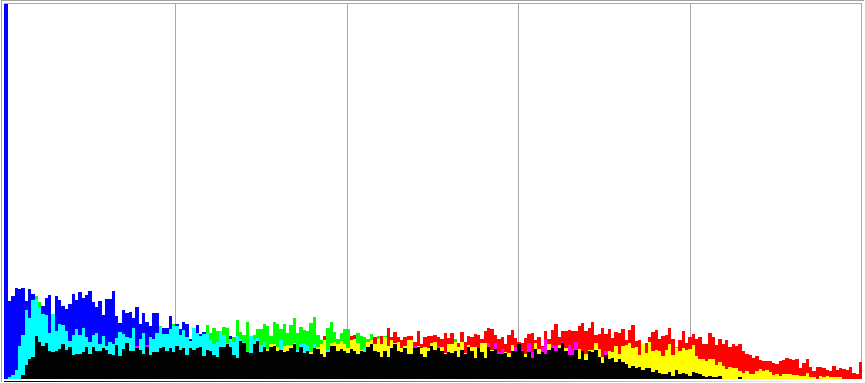
\includegraphics[width=\textwidth]{figures/tiger_smallHisto.png}
            \caption{Cover image}
            \label{fig:coverHisto}
    \end{subfigure}
    \begin{subfigure}[b]{0.49\textwidth}
            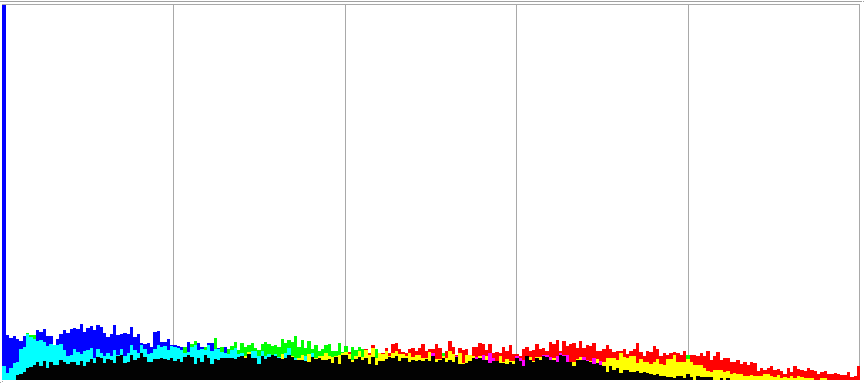
\includegraphics[width=\textwidth]{figures/gtOut2Histo.png}
            \caption{Cover image as JPEG}
            \label{fig:gt2Histo}
    \end{subfigure}
    \begin{subfigure}[b]{0.49\textwidth}
            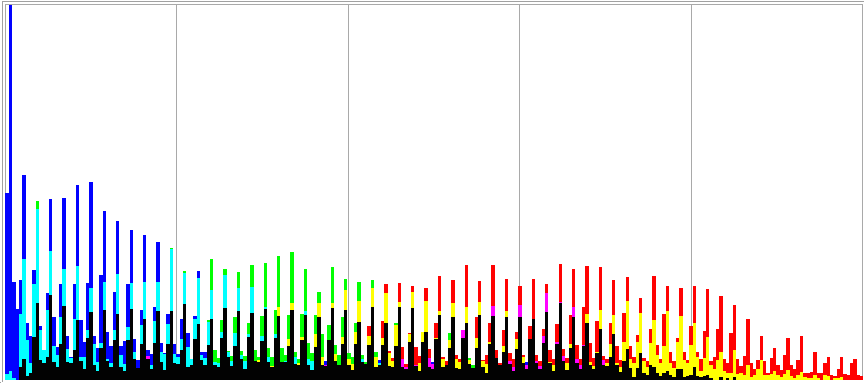
\includegraphics[width=\textwidth]{figures/lsbOutHisto.png}
            \caption{Stego image with message (LSB)}
            \label{fig:lsbHisto}
    \end{subfigure}
    \begin{subfigure}[b]{0.49\textwidth}
            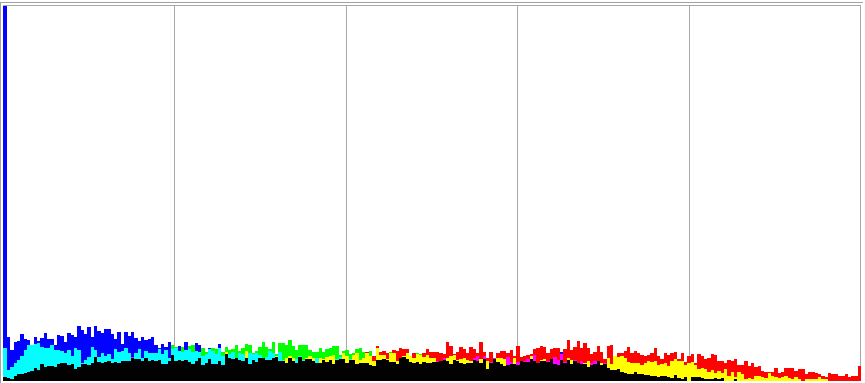
\includegraphics[width=\textwidth]{figures/gtOutHisto.png}
            \caption{Stego image with message (GT)}
            \label{fig:gtHisto}
    \end{subfigure}
    \caption{Histogram of a 120x120 px image}
    \label{fig:histogramsComparisons}
\end{figure}

In figure \ref{fig:histogramsComparisons} four histograms are shown.
Figures \ref{fig:coverHisto} and \ref{fig:gt2Histo} show the histogram of the original image and for the image encoded as JPEG without a message.
In figure \ref{fig:lsbHisto} and \ref{fig:gtHisto} the histograms of the images filled with a message using the LSB and GT methods respectively.
From these results it was clear that there was not much difference between the colour histograms of the image saved as JPEG with or without the message.
The image saved with LSB's histogram, however, clearly showed signs that the image had been tampered with.

The reason the histogram looked like that for the LSB image was because the bit-patterns of the encoded data became very clear in the histograms.
The bytes encoded in the images were the characters A-Z in ASCII repeated the capacity of the image had been reached.
A-Z in ASCII ranges from $65-90$, or in base two: $01000001_2-01011010_2$.
As the range was quite short, a lot of the higher order bits would rarely change, and those patterns became obvious in the histogram, as pixels ending in these patterns became more common.

The histogram in figure \ref{fig:lsbHisto} also showed how the LSB method changed images where a colour is very common.
The leftmost bar described pixels whose B-component is 0.
In the original cover image, this bar was much higher than the others, and therefore much more common in the image, but the LSB has made it so that those components now get spread out, which again becomes very obvious in the histogram.

\subsection{Euclidean distance}
A different way of looking for changes in an image is by looking at their Euclidean distance.
This can be done by calculating the distance between the colour values of each pixel in two equally sized images.
The sum of all these distances can be used as measure of the change from one image to the other.
We used this same method for determining what changes were imposed on images of different size and format, when uploaded to various social media and image-sharing websites.
The images used for the method were the same as those previously used in the colour histogram tests.
The results of these tests can be seen in table \ref {fig:euclidean_distance}.

\begin{table}[]
	\centering
	\begin{tabular}{@{}lllll@{}}
		\toprule
		\textbf{Images}            & \textbf{All channels} & \textbf{R} & \textbf{G} & \textbf{B} \\ \midrule
		\textit{Original and LSB}  & 34671                 & 17098      & 16800      & 16824      \\
		\textit{Original and GT}   & 130389                & 71112      & 56972      & 71886      \\
		\textit{Original and JPEG} & 102460                & 56758      & 40707      & 57569      \\
		\textit{JPEG and GT}       & 79163                 & 42154      & 38833      & 43217     
	\end{tabular}
	\caption{Calculated euclidean distances for several combinations of images.}
	\label{fig:euclidean_distance}
\end{table}


Comparing these results directly with the ones obtained from the LSB-method would be folly.
While the LSB-method might incur a smaller difference in the Euclidean distance it would not necessarily make it any better.

The other reason for the differences being larger is due to how the JPEG-file format is encoded.
Using the LSB of every pixel there is only the potential to change the value of each pixel by one.
Using the graph-theoretical approach with an M value of four, means that each individual value can be changed by four. 
This change is applied after the quantization step to avoid losing the data again.
This in turn means that the small change of up to four is multiplied by the quantization table, when the image is shown.
Bla bla something something green is less than the other

First of all using this method required that the user was in possession of both the original and the stego image.
This would indeed be possible if the parties sharing secret messages in the images, were using images they found on the internet and tampered with them.
Ths meant that they could completely foil any risk of being compromised by an outside party measuring euclidean distance, by simply using images that they took themselves.

So while the Euclidean distance might be bigger in the image where the data is hidden using our GT programme, it is of little use in automated system doing steganalysis on a multitude of images, as it would have nothing to compare the images to. 
Such a system could however check the histogram of the image, and discover abnormalities such as those the LSB method produces, as shown in figure \ref{fig:lsbHisto}.
	
\printbibliography[heading=bibintoc]
\label{bib:mybiblio}

\appendix
\chapter{Stego\_Image\_LSB}
%\label{ch:appAlabel}
\section*{BaseLSB}
\lstinputlisting[label={code:BaseLSB}, caption={BaseLSB class. Both EncodeLSB and DecodeLSB inherit from it.}]{../Programmer/Stego_Image_LSB/Stego_Image_LSB/BaseLSB.cs}
\section*{EncodeLSB}
\lstinputlisting[label={code:EncodeLSB}, caption={EncodeLSB class. The Class which encodes an image into its cover image.}]{../Programmer/Stego_Image_LSB/Stego_Image_LSB/EncodeLSB.cs}
\section*{DecodeLSB}
\lstinputlisting[label={code:DecodeLSB}, caption={DecodeLSB class. The Class which decodes an image from the cover image.}]{../Programmer/Stego_Image_LSB/Stego_Image_LSB/DecodeLSB.cs}
\section*{Program}
\lstinputlisting[label={code:Program}, caption={Where the program starts. It opens up the windows form, which allows users to encode/decode images.}]{../Programmer/Stego_Image_LSB/Stego_Image_LSB/Program.cs}
\section*{Windows Form}
\lstinputlisting[label={code:WindowsForms}, caption={The graphical user interface for the program}]{../Programmer/Stego_Image_LSB/TestForm/TestForm.cs}


\end{document}